\chapter{Preliminaries}\label{chapter:Preliminaries}
This chapter establishes a theoretical basis consisting of declarations and definitions required for the understanding of the ideas and their implementations proposed in this work. The four fields forming this basis are the representation of logic circuits (Section~\ref{sec:LogCirc}), QCA technology (Section~\ref{sec:QCATec}), the placement and routing problem (Section~\ref{sec:PR}) and sequentiality (Section~\ref{subsec:latchesandregisters}).

\section{Representation of logic circuits}\label{sec:LogCirc}
Logic circuits provide a powerful construct that allows an abstraction of digital circuits to a logic level and thereby makes it possible to discuss and argue about them scientifically. This abstraction was made possible by the Boolean algebra, formed by the mathematician George Boole in 1847. It shows that every digital circuit can be represented by logic functions, independent of their underlying technology \cite{halmos2009introduction}. In the following sections first, a definition of a Boolean algebra is given, and second, it is shown how logic networks can be formed using them.

\subsection{Boolean Functions}\label{subsec:boolfunc}
A definition of Boolean calculus was first provided by Edward V. Huntington in 1993. From \textit{set of independent postulates for the algebra of logic} and his own correction \cite{HuntingtonPostulate, HuntingtonCorrection}, the following equations form the basis of every Boolean algebra:

\begin{definition}[Basis for Boolean algebra]\label{Def:BasBool}
	Let $a, b, c$ be arbitrary elements of an abstract algebra $(L, +, ')$ with their set denoted as $B_{abc}$. The algebra includes the binary function disjunction $+ : B_{abc} \times B_{abc} \rightarrow B_{abc}$ and the unary function $' : B_{abc} \rightarrow B_{abc}$.
	\begin{table}[h]
		\centering
		\begin{tabular}{c}
			$a + b = b + a$ \\
			$(a + b) + c =  a + (b + c)$\\
			$(a' + b')' + (a' + b)' = a$\\
		\end{tabular}
	\end{table}
	
	The last of his postulates is named after the inventor and is commonly known as \textit{Huntington equation}. 
	\newpage
	There also exists an "universe element" $u \in B_{abc}$ for which holds:
	
	\begin{table}[h]
		\centering
		\begin{tabular}{l}
			$\exists u' : a + u' = a$ \\
			$\exists u : a + a' = u$. \\
		\end{tabular}
	\end{table}
	
\end{definition}

Despite the capability of the disjunction and negation operators to construct a Boolean algebra, it is common practice to additionally utilize the conjunction operator $\cdot : B_{abc} \times B_{abc} \rightarrow B_{abc}$ to create more concise and comprehensible logical expressions.
The most widely used Boolean algebra, denoted as $\mathbb{B}$, is defined as the tuple $(B_{abc}, \vee, \wedge, \neg)$, where $\vee$ and $\wedge$ are alternate notations for the binary disjunction operator $+$ and conjunction operator $\cdot$ within $\mathbb{B}$. The third function, $\neg$, represents the unary negation operation, previously denoted as $'$. The set $B_{abc}$ comprises of two distinct elements, namely ${0, 1}$, with $u=1$ and $\neg u = 0$ in accordance with the definition in \cite{Boolean_def}.

Given that this definition is limited to the utilization of only the three Boolean functions $(\vee, \wedge, \neg)$, an extension to this definition is proposed in \cite{muti_output_boolean_function}.

\begin{definition}[Boolean function]
	A Boolean function can be described as $f: \{0, 1\}^k \to \{0, 1\}$, with $k \in \mathbb{N}^*$ being the number of arguments or arity of the function. A function with $k$ arguments is referred to as $k$-ary. Multi-output Boolean functions can be described as $\{0, 1\}^k \to \{0, 1\}^m$, with $k \in \mathbb{N}^*$ and the integer $m > 0$.
\end{definition}

Nonetheless, every $k$-ary function can still be decomposed into a set of common Boolean functions $(\vee, \wedge, \neg )$. One example for this is the 3-ary majority function, which is a very important Boolean function for QCA technology.

\begin{definition}[Majority Function]\label{Def:majf}
	The ternary Boolean majority function is defined as: $\langle a, b, c \rangle = ab + ac + bc$, so that the function value equals the majority of it's incoming values.
	
	It follows: $\langle a, b, 0 \rangle = a \cdot b$ and $\langle a, b, 1 \rangle = a + b$.
\end{definition}

Common notations for Boolean functions are \textit{conjunctive normal form} (CNF) or \textit{disjunctive normal form} (DNF), using literals.

\begin{definition}[Literal]
	A literal is either an atom $a$ (positive literal) or the negation of an atom $\neg a$ (negative literal).
\end{definition}

\begin{definition}[CNF and DNF]
	A propositional Boolean formula is said to be in CNF if it is a conjunction of \textit{clauses}, each of which is a disjunction of literals \cite{CNF}:
	
	\[\displaystyle\bigwedge_{i} \displaystyle\bigvee_{j} (\neg) v_{ij}, \]
	where $v_{ij} \in \mathbb{B}$.
	
	A propositional Boolean formula is said to be in DNF if it is a disjunction of clauses, each of which is a conjunction of literals:
	
	\[ \displaystyle\bigvee_{i} \displaystyle\bigwedge_{j} (\neg) v_{ij}, \]
	where $v_{ij} \in \mathbb{B}$.
	
\end{definition}

Using the CNF or rather the DNF, Definition~\ref{Def:BasBool} and \textit{De Morgan's laws} \cite{DeMorgans_laws}:

\begin{definition}[De Morgan's laws]
	Given a Boolean Algebra $\mathbb{B} = (B_{ab}, \vee, \wedge, \neg)$ with two arbitrary elements $a,b \in B_{ab} = {0, 1}$, the following logic principles can be applied:
	\begin{table}[h]
		\centering
		\begin{tabular}{c}
			$\neg a \wedge \neg b = \neg (b \vee a)$ \\
			$\neg a \vee \neg b = \neg (b \wedge a)$,
		\end{tabular}
	\end{table}
\end{definition}

it follows that any Boolean algebra can be reduced to only two operands, e.g., conjunction ($\vee$) and negation ($\neg$) or disjunction ($\wedge$) and negation ($\neg$). Any set of such two Boolean functions is called \textit{universal}.

\subsection{Logic Networks}

There are many ways of representing Boolean Functions. But all \textit{canonical} forms like truth tables (TTs), reduced sum of products (RSOPs) or binary decision diagrams (BDDs), suffer from exponential representations, making them impractical for big logic circuits. Even if a reasonable representation exists for a given function, simple operations like forming the complementary could yield an exponential function representation \cite{canonical}.

Logic networks overcome these restrictions by being \textit{non-canonical}, meaning that a given function can be represented by different logic networks. The following definition for Logic Networks is derived from \cite{LogicNetwork}:

\begin{definition}[Logic Network]
	A logic network $N(V, E)$ is a rooted, directed graph with vertex set $V$ and edge set $E$. For any vertex $v \in V$, vertices connected by incoming edges $e_{inc} \in E$ are called parent. A vertex connected by an outgoing edge $e_{out} \in E$ is called child.
	$V$ contains two types of vertices. A \textit{non-terminal} vertex $v$ has as attributes an argument index $index(v) \in \{1, . . .,n\}$, and $l$ parents $parent_1(v), ..., parent_l(v) \in V$. 
	A \textit{terminal} vertex v has as attribute a value $value(v)\in\{0,1\}$.
	
	Furthermore, for any non-terminal vertex $v$, if $parent_i(v)$ with $ 1 \leq i \leq l$, then we must have $index(parent_i(v)) < index(parent_l(v))$ respectively.
\end{definition}

This definition allows vertices to have an unrestricted number of parents, implying that the Boolean function represented by the vertex can be $k$-ary:

\begin{definition}[Logic Network Boolean Functions]
	A set of $k$-ary Boolean Functions $x_1, ..., x_n \in \mathbb{B}$ is assigned to every vertex via the argument index $index(v) = i$. The graph function $f_v$ is defined recursively as:
	\begin{enumerate}
		\item If v is a terminal vertex:
		\begin{enumerate}
			\item If $value(v)=1$, then $f_v=1$
			\item If $value(v)=0$, then $f_v=0$
		\end{enumerate}
		\item If $v$ is a non-terminal vertex with $index(v)=i$, then $f_v$ is the function:
		
		$f_v(v_i) = x_i(f_{parent_1(v)}(v_{i-1}), ..., f_{parent_l(v)}(v_{i-n}))$.
	\end{enumerate}
\end{definition}

\begin{figure}
	\centering
	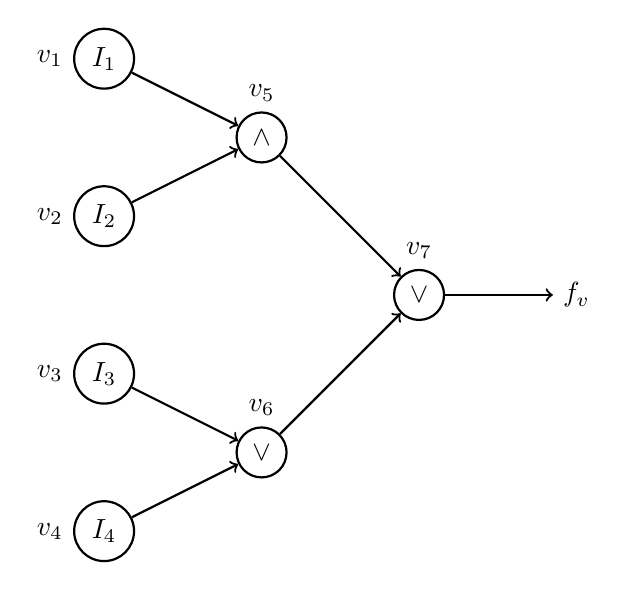
\begin{tikzpicture}[node distance={2cm and 2cm}, thick, main/.style = {draw, circle}] 
		\node[main] (1) at (0,0) [label=west:$v_1$]{$I_1$}; 
		\node[main] (2) at (0,-2)[label=west:$v_2$] {$I_2$};
		\node[main] (3) at (0,-4)[label=west:$v_3$] {$I_3$};
		\node[main] (4) at (0,-6)[label=west:$v_4$] {$I_4$}; 
		
		\node[main] (5) at (2,-1)[label=north:$v_5$]{$\wedge$}; 
		\node[main] (6) at (2,-5)[label=north:$v_6$]{$\vee$};
		
		\node[main] (7) at (4,-3)[label=north:$v_7$]{$\vee$};
		
		\node [right of = 7] (f) {$f_v$};
		
		
		\draw[->] (1) -- (5);
		\draw[->] (2) -- (5);
		\draw[->] (3) -- (6);
		\draw[->] (4) -- (6);
		\draw[->] (5) -- (7);
		\draw[->] (6) -- (7);
		\draw[->] (7) -- (f);
		
	\end{tikzpicture} 
	\\
	\hfill \break
	The corresponding recursive Boolean function reads:\\
	\hfill \break
	\begin{tabular}{l l}
		
		$f_v = f_v(v_7)$ &  $f_v(v_6) = f_v(v_3) \wedge f_v(v_4)$\\
		$f_v(v_7) = f_v(v_5) \vee f_v(v_6)$ &  $f_v(v_5) = f_v(v_1) \vee f_v(v_2)$\\
		&\\
		with primary inputs: & 	$f_v(v_1), f_v(v_2), f_v(v_3), f_v(v_4) \in \{0, 1\}$\\
		&\\
	\end{tabular}
	
	\caption{Binary Logic Network} \label{fig:LNEx}
\end{figure}

The recursive nature of the Boolean Function definition in logic networks can be seen in Figure~\ref{fig:LNEx}.

The non-canonical property can be explained by the fact that nodes with the identity function are allowed, which can be inserted everywhere in the logic network, while the function representation of the logic network stays the same. Even the exclusion of such identity nodes has no impact, since simple node combinations, like two negation nodes, collapse to the identity function. Following this argumentation, there exists an infinite number of logic networks representing each one Boolean Function, resulting in the widely accepted assumption, that the determination of an optimal logic network is an $\mathcal{NP}$-complete problem \cite{Walter}. Attempts to create canonical logic networks, seem to evade this problem, but include $co\mathcal{NP}$-complete problems in itself \cite{LogicNetwork}.
Nevertheless, logic networks have proven to be very useful in transforming logic circuits into gate representations. This process is called \textit{logic synthesis}. Due to the complexity of the representations algorithms commonly used for logic synthesis are based on approximate solutions.


%\begin{definition}[Function graph as BDD]
%	A function graph is a rooted, directed graph with vertex set $V$ containing two types of vertices. A \textit{non-terminal} vertex $v$ has as attributes an argument index $index(v) \in \{1, . . .,n\}$, and two children $low(v),high(v) \in V$. A \textit{terminal} vertex v has as attribute a value $value(v)\in\{0,1\}$.\\
%	\\
%	Furthermore, for any non-terminal vertex $v$, if $low(v)$ is also non-terminal, then we must have
%	$index(v) < index(low(v))$. Similarly, if $high(v)$ is non-terminal, then we must have
%	$index(v) < index(high(v))$.
%\end{definition}

%\begin{definition}[Function Graph Boolean Functions]
%	A function graph $G$ having root vertex $v$ denotes a function $f_v$ defined recursively as:
%	\begin{enumerate}
%		\item If v is a terminal vertex:
%		\begin{enumerate}
%			\item If $value(v)=1$, then $f_v=1$
%			\item If $value(v)=0$, then $f_v=0$
%		\end{enumerate}
%		\item If $v$ is a non-terminal vertex with $index(v)=i$, then $f_v$ is the function \\ 
%		$f_v(x_1, ..., x_n) = \bar{x}_i \cdot f_{low(v)}(x_1, ..., x_n) + x_i \cdot f_{high(v)}(x_1, ..., x_n)$.
%	\end{enumerate}
%\end{definition}

Adapting from the definitions in \cite{Walter}, a terminal vertex is referred to as \textit{primary input} (PI) with their set denoted as $I$. The set of non-terminal vertices referred to as \textit{nodes} is denoted as $\Lambda$. The definition requires $I \cap \Lambda = \emptyset$. An edge connecting a parent $\nu_i$ and a child vertex $\nu_j$ is called a \textit{signal}. With $i < j$ the notation of a signal is given as $(\nu_i, \nu_j)$. The set of all signals is denoted as $\Sigma$. If an edge is dangling, so it doesn't point to another vertex, it is called \textit{primary output} (PO) and their set is denoted as $O$. Therefore also $\Sigma \cap O = \emptyset$ holds. From the definition of a logic network, we can now describe it as acyclic directed graph $N = (\Lambda, I, \Sigma, O)$.

As already mentioned in Section~\ref{subsec:boolfunc}, a universal set of two Boolean functions can form any Boolean algebra.
As long as this universality is contained, the set of node functions in a logic network can be extended arbitrarily. Common logic networks containing only two network functions are e.g. \textit{AND-Inverter Graphs} (AIGs) \cite{bandyopadhyay2019design} allowing only conjunction and negation. Another binary logic network, which is used in the QCA domain, is the \textit{Majority-Inverter Graphs} (MIGs) \cite{bandyopadhyay2019design} utilizing the ternary majority function and negation. But there also exists a wide range of logic networks that permit more than just two-node functions. One example is the \textit{AND-OR-Inverter Graph} (AOIG) with conjunction, disjunction, and negation functions, respectively \cite{Walter}.

As part of the logic synthesis, a suitable logic network representation of the combinational circuit has to be determined. Because, even though these logic networks can implement any Boolean function given by a specification, not every logic network can be synthesized into any given technology.
Looking at the current standard technology \textit{complementary metal-oxidesemiconductor} (CMOS), the logic network is then synthesized by using building blocks consisting of \textit{metal-oxide-semiconductor field-effect transistors} (MOSFETs), the elemental unit in this technology.

\section{QCA Technology}\label{sec:QCATec}

In order to fulfill the well-known Moore's law \cite{Moores_Law}, demanding a doubling of transistors on a chip every two years, CMOS technology is facing a multitude of challenges. Most notable are the short-channel effect, impurity variations, and most importantly, the heat dissipation resulting from static and dynamic power losses \cite{challenges_1, challenges_2, challenges_3}. To tackle these challenges among others the International Roadmap for Devices and Systems (IRDS, former by ITRS), provides a platform proposing solutions within the semiconductor domain, e.g. new materials and multi-core architectures. Also new technologies are being researched, including quantum computing and the domain of \textit{Field-Coupled Nanocomputing} (FCN) \cite{safoev2020design}. This work focuses on one of the most promising FCN technologies, namely \textit{Quantum-dot Cellular Automata} (QCA). The main difference of this technology compared to CMOS is the representation of logical modes, using the location of electron pairs in QCA-cells, rather than voltage levels. Data between cells are transferred based on Coulomb repulsion, using electromagnetic fields, enabling the technology to achieve high performance in terms of device density, clock frequency, and power consumption \cite{mohammadi2016efficient}. Hence, QCA tackles exactly the main issues faced by CMOS technology and provides a promising digital system for the future \cite{ahmad2018optimal}. However, QCA also presents its own challenges in terms of the manufacturing process, manufacturing standards, and different design
methodologies \cite{Bennet_waveform}. Because this work focuses on the design of QCA circuits, it mainly views circuit parameters such as area, performance, and wire crossings \cite{ahmad2018optimal}. In order to allow an analysis under these parameters, first the QCA technology and the resulting design constraints have to be understood. Therefore, Section~\ref{subsec:cells} introduces QCA cells as building blocks for QCA gates, which are discussed in Section~\ref{subsec:gates}. After understanding the clocking in Section~\ref{subsec:clocking}, the constraints for the placement and routing problem can be formulated subsequently. In addition sequential behavior is discussed in CMOS and transferred to the QCA domain in Section~\ref{subsec:latchesandregisters}.

\subsection{Cells}\label{subsec:cells}

As already mentioned, in QCA technology logical states are no longer represented by voltage levels but by the location of electrons \cite{QCA_technology}. In order to achieve this property a nanosized structure is needed, which is capable of trapping electrons in a certain position. The utilization of so-called \emph{quantum-dots} (QDs) serves as the foundation for this study. QDs can be implemented in various ways, including the use of several to one hundred atoms of a semiconductor in CMOS-QCA technology \cite{Quantum_dots}, the implementation of nanomagnets in mQCA technology \cite{orlov2008magnetic}, or the use of patterned dangling bonds on hydrogen passivated silicon referred to as SiDBs \cite{retallick2020population}. As a result, quantum mechanics applies to the electrical properties of QDs. For this work it is sufficient to understand that every QD has a bound state, where a particle tends to be localized and the bound state is subject to a potential, which can be external or due to the presence of other particles. Because this enables QDs to have discrete electronic states, they are also referred to as \textit{artificial atoms}. A combination of them is used to build a QCA cell, also known as \textit{artificial molecule} \cite{Quantum_dots}. Figure~\ref{fig:QCAStates} shows three such QCA cells, where the four circles at the corners of each QCA cell represent the QDs or rather their quantum barriers, which are capable of trapping each one electron. In addition, a cell contains two excess electrons, which can be localized by quantum dots. When a QD currently traps an electron, it is depicted black and an unoccupied QD is depicted white. Coulomb repulsion causes electrons to occupy diagonally opposed QDs, resulting in three possible cell states \cite{Sasamal2020QuantumDotCA, lent1997device, lent1994quantum}.

A stable state indicates that it is easily distinguishable from the usual energy band. Therefore, the energy difference between two consecutive energy states must be well above the thermal noise energy ($k_BT$). Only such states are suited for information transfer. The stable states can be derived from cell polarization, which can be $+1$ and $-1$ or $null$ in the unexcited state. The two stable states contain the same electrostatic energy and are used to encode the binary values $0$ and $1$ \cite{Sasamal2020QuantumDotCA}. Figure~\ref{fig:QCAStates} shows three cells with possible states and their resulting polarizations and logical states.

As already stated, QDs can be influenced externally, allowing the designer to fix the polarization of a QCA cell. This effect is used to input information into one QCA cell, called the driver cell. When a driver cell is placed side-by-side with other QCA cells, its polarization causes the polarization of the adjacent cell to change. When the adjacent cell is polarized, it passes its state again to the next cell and so on \cite{lent1997device}. Figure~\ref{fig:QCAWire} depicts such a structure, where the left-most cell represents the driver cell with fixed polarization representing a logic "1". With every cell passing its polarization to the cell to its right, the polarization of the right-most cell can be measured and the logic value, which propagated through the structure can be extracted. Due to the property of just passing the information from its input to its output, the shown structure represents a QCA wire segment.

\begin{figure}
	\centering
	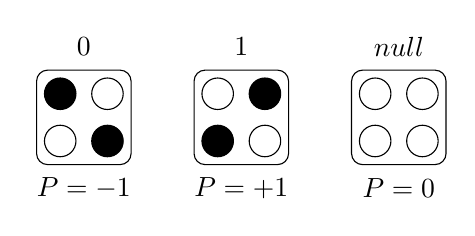
\begin{tikzpicture}
		%One QCA-Cell
		\node (A1) at (0.6,1.5) {$0$};
		\draw[rounded corners] (0, 0) rectangle (1.2, 1.2) [label=north:$v_7$]{};
		\node (A2) at (0.6,-0.3) {$P = -1$};
		
		\draw (0.3,0.3) circle (2mm);
		\draw [fill = black] (0.9,0.3) circle (2mm);
		\draw [fill = black](0.3,0.9) circle (2mm);
		\draw (0.9,0.9) circle (2mm);
		
		
		%One QCA-Cell
		\def\x{2}
		\node (B1) at (0.6+\x,1.5) {$1$};
		\draw[rounded corners] (\x, 0) rectangle (1.2 + \x, 1.2) {};
		\node (B2) at (0.6+\x,-0.3) {$P = +1$};
	
		\draw [fill = black] (0.3+\x,0.3) circle (2mm);
		\draw (0.9+\x,0.3) circle (2mm);
		\draw (0.3+\x,0.9) circle (2mm);
		\draw [fill = black] (0.9+\x,0.9) circle (2mm);
		
		
		%One QCA-Cell
		\def\x{4}
		\node (C1) at (0.6+\x,1.5) {$null$};
		\draw[rounded corners] (\x, 0) rectangle (1.2 + \x, 1.2) {};
		\node (C2) at (0.6+\x,-0.3) {$P = 0$};
		
		\draw (0.3+\x,0.3) circle (2mm);
		\draw (0.9+\x,0.3) circle (2mm);
		\draw (0.3+\x,0.9) circle (2mm);
		\draw (0.9+\x,0.9) circle (2mm);
		
		
	\end{tikzpicture} 

	\caption{QCA-Cell sates} \label{fig:QCAStates}
\end{figure}

\begin{figure}
	\centering
	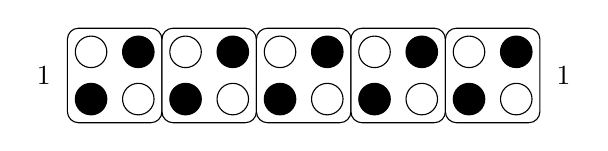
\begin{tikzpicture}
		%One QCA-Cell
		\node (A1) at (-0.3,0.6) {$1$};
		\draw[rounded corners] (0, 0) rectangle (1.2, 1.2) [label=north:$v_7$]{};
		
		\draw [fill = black](0.3,0.3) circle (2mm);
		\draw (0.9,0.3) circle (2mm);
		\draw (0.3,0.9) circle (2mm);
		\draw [fill = black](0.9,0.9) circle (2mm);
		
		
		%One QCA-Cell
		\def\x{1.2}
		\draw[rounded corners] (\x, 0) rectangle (1.2 + \x, 1.2) {};
		
		\draw [fill = black] (0.3+\x,0.3) circle (2mm);
		\draw (0.9+\x,0.3) circle (2mm);
		\draw (0.3+\x,0.9) circle (2mm);
		\draw [fill = black] (0.9+\x,0.9) circle (2mm);
		
		
		%One QCA-Cell
		\def\x{2.4}
		\draw[rounded corners] (\x, 0) rectangle (1.2 + \x, 1.2) {};
		\draw [fill = black](0.3+\x,0.3) circle (2mm);
		\draw (0.9+\x,0.3) circle (2mm);
		\draw (0.3+\x,0.9) circle (2mm);
		\draw [fill = black](0.9+\x,0.9) circle (2mm);
		
		%One QCA-Cell
		\def\x{3.6}
		\draw[rounded corners] (\x, 0) rectangle (1.2 + \x, 1.2) {};
		\draw [fill = black](0.3+\x,0.3) circle (2mm);
		\draw (0.9+\x,0.3) circle (2mm);
		\draw (0.3+\x,0.9) circle (2mm);
		\draw [fill = black](0.9+\x,0.9) circle (2mm);
		
		%One QCA-Cell
		\def\x{4.8}
		\draw[rounded corners] (\x, 0) rectangle (1.2 + \x, 1.2) {};
		\draw [fill = black](0.3+\x,0.3) circle (2mm);
		\draw (0.9+\x,0.3) circle (2mm);
		\draw (0.3+\x,0.9) circle (2mm);
		\draw [fill = black](0.9+\x,0.9) circle (2mm);
		\node (C1) at (1.5+\x,0.6) {$1$};
		
		
	\end{tikzpicture} 
	
	\caption{Adjacent QCA-cells forming a wire segment} \label{fig:QCAWire}
\end{figure}

\subsection{Gates}\label{subsec:gates}

In this subsection, QCA cells are combined to form different logic gates, which form the gate library used later for the design of QCA logical circuits. Some of these gates are inherited from the QCA ONE library \cite{QCA_scl}, which is already used fully \cite{peng2020spars} or partially \cite{ortho, fontes} as a basis for some existing works.

The QCA ONE library proposes gates formed by one tile as well as gates formed by multiple tiles. A tile describes a uniform size of gates. For the QCA ONE library a tile is of dimension $5 \times 5$ cells. A major drawback of this library is the use of some gates that are highly prone to crosstalk and the implementation of sequential circuits that do not align with the theory of this work \cite{QCA_scl}. Therefore, the gate library used in this work is presented below. The sequential theory is provided in Section~\ref{subsec:latchesandregisters}.
%%%%%%Inverter
\begin{figure}
	\centering
	\subfigure[Diagonal Inverter]
	{
		\centering
		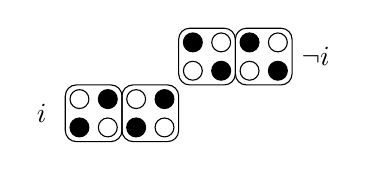
\begin{tikzpicture}
			%One QCA-Cell
			\node (A1) at (-0.3,0.36) {$i$};
			\draw[rounded corners] (0, 0) rectangle (1.2*0.6, 1.2*0.6) [label=north:$v_7$]{};
			
			\draw [fill = black](0.3*0.6,0.3*0.6) circle (2*0.6mm);
			\draw (0.9*0.6,0.3*0.6) circle (2*0.6mm);
			\draw (0.3*0.6,0.9*0.6) circle (2*0.6mm);
			\draw [fill = black](0.9*0.6,0.9*0.6) circle (2*0.6mm);
			
			
			%One QCA-Cell
			\def\x{0.72}
			\draw[rounded corners] (\x, 0) rectangle (1.2*0.6 + \x, 1.2*0.6) {};
			
			\draw [fill = black] (0.3*0.6+\x,0.3*0.6) circle (2*0.6mm);
			\draw (0.9*0.6+\x,0.3*0.6) circle (2*0.6mm);
			\draw (0.3*0.6+\x,0.9*0.6) circle (2*0.6mm);
			\draw [fill = black] (0.9*0.6+\x,0.9*0.6) circle (2*0.6mm);
			
			
			%One QCA-Cell
			\def\o{0.72}
			\def\x{1.44}
			\draw[rounded corners] (\x, 0 + \o) rectangle (1.2*0.6 + \x, 1.2*0.6 +\o) {};
			\draw (0.3*0.6+\x,0.3*0.6+\o) circle (2*0.6mm);
			\draw [fill = black](0.9*0.6+\x,0.3*0.6+\o) circle (2*0.6mm);
			\draw [fill = black](0.3*0.6+\x,0.9*0.6+\o) circle (2*0.6mm);
			\draw (0.9*0.6+\x,0.9*0.6+\o) circle (2*0.6mm);
			
			%One QCA-Cell
			\def\o{0.72}
			\def\x{2.16}
			\draw[rounded corners] (\x, 0+\o) rectangle (1.2*0.6 + \x, 1.2*0.6+\o) {};
			\draw (0.3*0.6+\x,0.3*0.6+\o) circle (2*0.6mm);
			\draw [fill = black](0.9*0.6+\x,0.3*0.6+\o) circle (2*0.6mm);
			\draw [fill = black](0.3*0.6+\x,0.9*0.6+\o) circle (2*0.6mm);
			\draw (0.9*0.6+\x,0.9*0.6+\o) circle (2*0.6mm);
			
			\node (C1) at (0.72 + \x + 0.3, 0.36+\o) {$\neg i$};
			
		\end{tikzpicture} 
		\label{subfig:45Inverter}
	}
	\subfigure[Standard Inverter]
	{
		\centering
		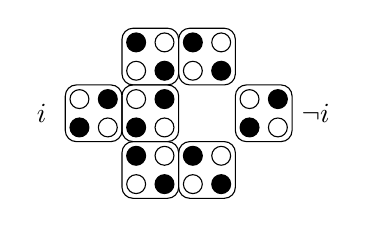
\begin{tikzpicture}
			%One QCA-Cell
			\node (A1) at (-0.3,0.36) {$i$};
			\draw[rounded corners] (0, 0) rectangle (1.2*0.6, 1.2*0.6) [label=north:$v_7$]{};
			
			\draw [fill = black](0.3*0.6,0.3*0.6) circle (2*0.6mm);
			\draw (0.9*0.6,0.3*0.6) circle (2*0.6mm);
			\draw (0.3*0.6,0.9*0.6) circle (2*0.6mm);
			\draw [fill = black](0.9*0.6,0.9*0.6) circle (2*0.6mm);
			
			
			%One QCA-Cell
			\def\x{0.72}
			\draw[rounded corners] (\x, 0) rectangle (1.2*0.6 + \x, 1.2*0.6) {};
			
			\draw [fill = black] (0.3*0.6+\x,0.3*0.6) circle (2*0.6mm);
			\draw (0.9*0.6+\x,0.3*0.6) circle (2*0.6mm);
			\draw (0.3*0.6+\x,0.9*0.6) circle (2*0.6mm);
			\draw [fill = black] (0.9*0.6+\x,0.9*0.6) circle (2*0.6mm);
			
			
			%One QCA-Cell
			\def\o{0.72}
			\def\x{0.72}
			\draw[rounded corners] (\x, 0 + \o) rectangle (1.2*0.6 + \x, 1.2*0.6 +\o) {};
			\draw (0.3*0.6+\x,0.3*0.6+\o) circle (2*0.6mm);
			\draw [fill = black](0.9*0.6+\x,0.3*0.6+\o) circle (2*0.6mm);
			\draw [fill = black](0.3*0.6+\x,0.9*0.6+\o) circle (2*0.6mm);
			\draw (0.9*0.6+\x,0.9*0.6+\o) circle (2*0.6mm);
			
			%One QCA-Cell
			\def\o{0.72}
			\def\x{1.44}
			\draw[rounded corners] (\x, 0+\o) rectangle (1.2*0.6 + \x, 1.2*0.6+\o) {};
			\draw (0.3*0.6+\x,0.3*0.6+\o) circle (2*0.6mm);
			\draw [fill = black](0.9*0.6+\x,0.3*0.6+\o) circle (2*0.6mm);
			\draw [fill = black](0.3*0.6+\x,0.9*0.6+\o) circle (2*0.6mm);
			\draw (0.9*0.6+\x,0.9*0.6+\o) circle (2*0.6mm);
			
			%One QCA-Cell
			\def\o{-0.72}
			\def\x{0.72}
			\draw[rounded corners] (\x, 0 + \o) rectangle (1.2*0.6 + \x, 1.2*0.6 +\o) {};
			\draw (0.3*0.6+\x,0.3*0.6+\o) circle (2*0.6mm);
			\draw [fill = black](0.9*0.6+\x,0.3*0.6+\o) circle (2*0.6mm);
			\draw [fill = black](0.3*0.6+\x,0.9*0.6+\o) circle (2*0.6mm);
			\draw (0.9*0.6+\x,0.9*0.6+\o) circle (2*0.6mm);
			
			%One QCA-Cell
			\def\o{-0.72}
			\def\x{1.44}
			\draw[rounded corners] (\x, 0+\o) rectangle (1.2*0.6 + \x, 1.2*0.6+\o) {};
			\draw (0.3*0.6+\x,0.3*0.6+\o) circle (2*0.6mm);
			\draw [fill = black](0.9*0.6+\x,0.3*0.6+\o) circle (2*0.6mm);
			\draw [fill = black](0.3*0.6+\x,0.9*0.6+\o) circle (2*0.6mm);
			\draw (0.9*0.6+\x,0.9*0.6+\o) circle (2*0.6mm);
			
			%One QCA-Cell
			\def\x{2.16}
			\draw[rounded corners] (\x, 0) rectangle (1.2*0.6 + \x, 1.2*0.6) {};
			
			\draw [fill = black] (0.3*0.6+\x,0.3*0.6) circle (2*0.6mm);
			\draw (0.9*0.6+\x,0.3*0.6) circle (2*0.6mm);
			\draw (0.3*0.6+\x,0.9*0.6) circle (2*0.6mm);
			\draw [fill = black] (0.9*0.6+\x,0.9*0.6) circle (2*0.6mm);
			
			\node (C1) at (0.72 + \x + 0.3, 0.36) {$\neg i$};
		\end{tikzpicture} 
		\label{subfig:StandardInverter}
	}
	\caption{Different QCA Inverter representations} \label{fig:QCAInverter}
\end{figure}

Inverters and majority gates are the main building blocks of QCA circuits. Starting with the inverter or NOT gate, the simplest implementation is shown in Figure~\ref{subfig:45Inverter}. It consists of two wire segments which are shifted by exactly one cell height, so that the polarization is transferred diagonally resulting in an inversion of the input \cite{Sasamal2020QuantumDotCA}. In order to get a more robust gate regarding disturbance, the C-shaped inverter shown in Figure~\ref{subfig:StandardInverter} was introduced \cite{QCA_scl}. This gate is used as standard in many libraries and works \cite{peng2020spars, fontes, sequential_cell_one, USE}, but it should be mentioned that this implementation is really prone to complex single-electron faults \cite{SingelElectronFaults} and even common displacement faults \cite{Inverter_displacements}, suggesting the addition of an inverter leg that results in an E-shaped gate structure. Nevertheless the C-shaped inverter gate is part of the QCA ONE library and is also selected as standard gate for this work.
%%%%%Majority gates
\begin{figure}
	\centering
	\subfigure[Rotated Majority gate]
	{
		\centering
		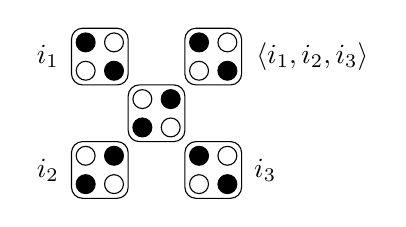
\begin{tikzpicture}
			%One QCA-Cell
			\node (I2) at (-0.3,0.36) {$i_2$};
			\draw[rounded corners] (0, 0) rectangle (1.2*0.6, 1.2*0.6) [label=north:$v_7$]{};
			
			\draw [fill = black](0.3*0.6,0.3*0.6) circle (2*0.6mm);
			\draw (0.9*0.6,0.3*0.6) circle (2*0.6mm);
			\draw (0.3*0.6,0.9*0.6) circle (2*0.6mm);
			\draw [fill = black](0.9*0.6,0.9*0.6) circle (2*0.6mm);
			
			%One QCA-Cell
			\def\o{0.72}
			\def\x{0.72}
			\draw[rounded corners] (\x, 0 + \o) rectangle (1.2*0.6 + \x, 1.2*0.6 +\o) {};
			\draw [fill = black](0.3*0.6+\x,0.3*0.6+\o) circle (2*0.6mm);
			\draw (0.9*0.6+\x,0.3*0.6+\o) circle (2*0.6mm);
			\draw (0.3*0.6+\x,0.9*0.6+\o) circle (2*0.6mm);
			\draw [fill = black](0.9*0.6+\x,0.9*0.6+\o) circle (2*0.6mm);
			
			%One QCA-Cell
			\def\o{1.44}
			\def\x{0}
			\node (I1) at (-0.3,0.36+\o) {$i_1$};
			\draw[rounded corners] (\x, 0+\o) rectangle (1.2*0.6 + \x, 1.2*0.6+\o) {};
			\draw (0.3*0.6+\x,0.3*0.6+\o) circle (2*0.6mm);
			\draw [fill = black](0.9*0.6+\x,0.3*0.6+\o) circle (2*0.6mm);
			\draw [fill = black](0.3*0.6+\x,0.9*0.6+\o) circle (2*0.6mm);
			\draw (0.9*0.6+\x,0.9*0.6+\o) circle (2*0.6mm);
			
			%One QCA-Cell
			\def\o{0}
			\def\x{1.44}
			\draw[rounded corners] (\x, 0 + \o) rectangle (1.2*0.6 + \x, 1.2*0.6 +\o) {};
			\draw (0.3*0.6+\x,0.3*0.6+\o) circle (2*0.6mm);
			\draw [fill = black](0.9*0.6+\x,0.3*0.6+\o) circle (2*0.6mm);
			\draw [fill = black](0.3*0.6+\x,0.9*0.6+\o) circle (2*0.6mm);
			\draw (0.9*0.6+\x,0.9*0.6+\o) circle (2*0.6mm);
			
			\node (I3) at (0.72 + \x + 0.3, 0.36+\o) {$i_3$};
			
			%One QCA-Cell
			\def\o{1.44}
			\def\x{1.44}
			\draw[rounded corners] (\x, 0+\o) rectangle (1.2*0.6 + \x, 1.2*0.6+\o) {};
			\draw (0.3*0.6+\x,0.3*0.6+\o) circle (2*0.6mm);
			\draw [fill = black](0.9*0.6+\x,0.3*0.6+\o) circle (2*0.6mm);
			\draw [fill = black](0.3*0.6+\x,0.9*0.6+\o) circle (2*0.6mm);
			\draw (0.9*0.6+\x,0.9*0.6+\o) circle (2*0.6mm);
			
			\node (C1) at (0.72 + \x + 0.9, 0.36+\o) {$\langle i_1, i_2, i_3\rangle$};
			
		\end{tikzpicture} 
		\label{subfig:rotatedMaj}
	}
	\subfigure[Standard Majority Gate]
	{
		\centering
		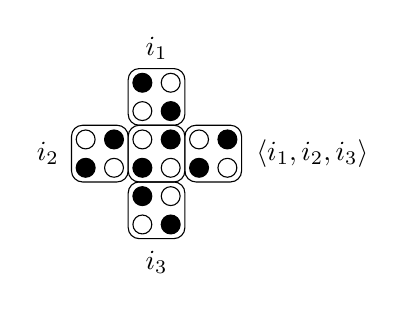
\begin{tikzpicture}
			%One QCA-Cell
			\node (I2) at (-0.3,0.36) {$i_2$};
			\draw[rounded corners] (0, 0) rectangle (1.2*0.6, 1.2*0.6) [label=north:$v_7$]{};
			
			\draw [fill = black](0.3*0.6,0.3*0.6) circle (2*0.6mm);
			\draw (0.9*0.6,0.3*0.6) circle (2*0.6mm);
			\draw (0.3*0.6,0.9*0.6) circle (2*0.6mm);
			\draw [fill = black](0.9*0.6,0.9*0.6) circle (2*0.6mm);
			
			
			%One QCA-Cell
			\def\x{0.72}
			\draw[rounded corners] (\x, 0) rectangle (1.2*0.6 + \x, 1.2*0.6) {};
			
			\draw [fill = black] (0.3*0.6+\x,0.3*0.6) circle (2*0.6mm);
			\draw (0.9*0.6+\x,0.3*0.6) circle (2*0.6mm);
			\draw (0.3*0.6+\x,0.9*0.6) circle (2*0.6mm);
			\draw [fill = black] (0.9*0.6+\x,0.9*0.6) circle (2*0.6mm);
			
			%One QCA-Cell
			\def\o{0.72}
			\def\x{0.72}
			\draw[rounded corners] (\x, 0 + \o) rectangle (1.2*0.6 + \x, 1.2*0.6 +\o) {};
			\draw (0.3*0.6+\x,0.3*0.6+\o) circle (2*0.6mm);
			\draw [fill = black](0.9*0.6+\x,0.3*0.6+\o) circle (2*0.6mm);
			\draw [fill = black](0.3*0.6+\x,0.9*0.6+\o) circle (2*0.6mm);
			\draw (0.9*0.6+\x,0.9*0.6+\o) circle (2*0.6mm);
			\node (I2) at (0.36 + \x,1.7) {$i_1$};
			
			
			%One QCA-Cell
			\def\o{-0.72}
			\def\x{0.72}
			\draw[rounded corners] (\x, 0 + \o) rectangle (1.2*0.6 + \x, 1.2*0.6 +\o) {};
			\draw (0.3*0.6+\x,0.3*0.6+\o) circle (2*0.6mm);
			\draw [fill = black](0.9*0.6+\x,0.3*0.6+\o) circle (2*0.6mm);
			\draw [fill = black](0.3*0.6+\x,0.9*0.6+\o) circle (2*0.6mm);
			\draw (0.9*0.6+\x,0.9*0.6+\o) circle (2*0.6mm);
			\node (I2) at (0.36 + \x,-1.02) {$i_3$};
			
			%One QCA-Cell
			\def\x{1.44}
			\draw[rounded corners] (\x, 0) rectangle (1.2*0.6 + \x, 1.2*0.6) {};
			
			\draw [fill = black] (0.3*0.6+\x,0.3*0.6) circle (2*0.6mm);
			\draw (0.9*0.6+\x,0.3*0.6) circle (2*0.6mm);
			\draw (0.3*0.6+\x,0.9*0.6) circle (2*0.6mm);
			\draw [fill = black] (0.9*0.6+\x,0.9*0.6) circle (2*0.6mm);
			
			\node (C1) at (0.72 + \x + 0.9, 0.36) {$\langle i_1, i_2, i_3\rangle$};
		\end{tikzpicture} 
		\label{subfig:StandardMaj}
	}\\
	\subfigure[Standard AND Gate]
	{
		\centering
		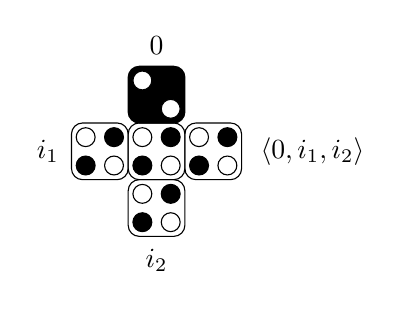
\begin{tikzpicture}
			%One QCA-Cell
			\node (I2) at (-0.3,0.36) {$i_1$};
			\draw[rounded corners] (0, 0) rectangle (1.2*0.6, 1.2*0.6) [label=north:$v_7$]{};
			
			\draw [fill = black](0.3*0.6,0.3*0.6) circle (2*0.6mm);
			\draw (0.9*0.6,0.3*0.6) circle (2*0.6mm);
			\draw (0.3*0.6,0.9*0.6) circle (2*0.6mm);
			\draw [fill = black](0.9*0.6,0.9*0.6) circle (2*0.6mm);
			
			
			%One QCA-Cell
			\def\x{0.72}
			\draw[rounded corners] (\x, 0) rectangle (1.2*0.6 + \x, 1.2*0.6) {};
			
			\draw [fill = black] (0.3*0.6+\x,0.3*0.6) circle (2*0.6mm);
			\draw (0.9*0.6+\x,0.3*0.6) circle (2*0.6mm);
			\draw (0.3*0.6+\x,0.9*0.6) circle (2*0.6mm);
			\draw [fill = black] (0.9*0.6+\x,0.9*0.6) circle (2*0.6mm);
			
			%One QCA-Cell
			\def\o{0.72}
			\def\x{0.72}
			\draw[rounded corners, fill=black] (\x, 0 + \o) rectangle (1.2*0.6 + \x, 1.2*0.6 +\o) {};
			\draw (0.3*0.6+\x,0.3*0.6+\o) circle (2*0.6mm);
			\draw [fill = white](0.9*0.6+\x,0.3*0.6+\o) circle (2*0.6mm);
			\draw [fill = white](0.3*0.6+\x,0.9*0.6+\o) circle (2*0.6mm);
			\draw (0.9*0.6+\x,0.9*0.6+\o) circle (2*0.6mm);
			\node (I2) at (0.36 + \x,1.7) {$0$};
			
			
			%One QCA-Cell
			\def\o{-0.72}
			\def\x{0.72}
			\draw[rounded corners] (\x, 0 + \o) rectangle (1.2*0.6 + \x, 1.2*0.6 +\o) {};
			\draw [fill = black](0.3*0.6+\x,0.3*0.6+\o) circle (2*0.6mm);
			\draw (0.9*0.6+\x,0.3*0.6+\o) circle (2*0.6mm);
			\draw (0.3*0.6+\x,0.9*0.6+\o) circle (2*0.6mm);
			\draw [fill = black](0.9*0.6+\x,0.9*0.6+\o) circle (2*0.6mm);
			\node (I2) at (0.36 + \x,-1.02) {$i_2$};
			
			%One QCA-Cell
			\def\x{1.44}
			\draw[rounded corners] (\x, 0) rectangle (1.2*0.6 + \x, 1.2*0.6) {};
			
			\draw [fill = black] (0.3*0.6+\x,0.3*0.6) circle (2*0.6mm);
			\draw (0.9*0.6+\x,0.3*0.6) circle (2*0.6mm);
			\draw (0.3*0.6+\x,0.9*0.6) circle (2*0.6mm);
			\draw [fill = black] (0.9*0.6+\x,0.9*0.6) circle (2*0.6mm);
			
			\node (C1) at (0.72 + \x + 0.9, 0.36) {$\langle 0, i_1, i_2\rangle$};
		\end{tikzpicture}
		\label{subfig:StandardAnd}
	}
	\subfigure[Standard OR Gate]
	{
		\centering
		 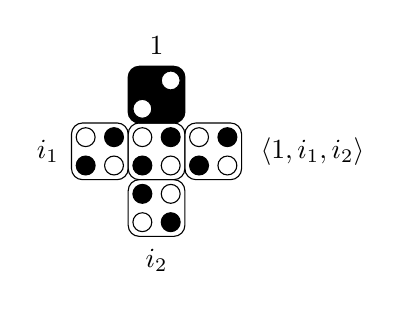
\begin{tikzpicture}
		 	%One QCA-Cell
		 	\node (I2) at (-0.3,0.36) {$i_1$};
		 	\draw[rounded corners] (0, 0) rectangle (1.2*0.6, 1.2*0.6) [label=north:$v_7$]{};
		 	
		 	\draw [fill = black](0.3*0.6,0.3*0.6) circle (2*0.6mm);
		 	\draw (0.9*0.6,0.3*0.6) circle (2*0.6mm);
		 	\draw (0.3*0.6,0.9*0.6) circle (2*0.6mm);
		 	\draw [fill = black](0.9*0.6,0.9*0.6) circle (2*0.6mm);
		 	
		 	%One QCA-Cell
		 	\def\x{0.72}
		 	\draw[rounded corners] (\x, 0) rectangle (1.2*0.6 + \x, 1.2*0.6) {};
		 	
		 	\draw [fill = black] (0.3*0.6+\x,0.3*0.6) circle (2*0.6mm);
		 	\draw (0.9*0.6+\x,0.3*0.6) circle (2*0.6mm);
		 	\draw (0.3*0.6+\x,0.9*0.6) circle (2*0.6mm);
		 	\draw [fill = black] (0.9*0.6+\x,0.9*0.6) circle (2*0.6mm);
		 	
		 	%One QCA-Cell
		 	\def\o{0.72}
		 	\def\x{0.72}
		 	\draw[rounded corners, fill=black] (\x, 0 + \o) rectangle (1.2*0.6 + \x, 1.2*0.6 +\o) {};
		 	\draw [fill = white](0.3*0.6+\x,0.3*0.6+\o) circle (2*0.6mm);
		 	\draw (0.9*0.6+\x,0.3*0.6+\o) circle (2*0.6mm);
		 	\draw (0.3*0.6+\x,0.9*0.6+\o) circle (2*0.6mm);
		 	\draw [fill = white](0.9*0.6+\x,0.9*0.6+\o) circle (2*0.6mm);
		 	\node (I2) at (0.36 + \x,1.7) {$1$};
		 	
		 	
		 	%One QCA-Cell
		 	\def\o{-0.72}
		 	\def\x{0.72}
		 	\draw[rounded corners] (\x, 0 + \o) rectangle (1.2*0.6 + \x, 1.2*0.6 +\o) {};
		 	\draw (0.3*0.6+\x,0.3*0.6+\o) circle (2*0.6mm);
		 	\draw [fill = black](0.9*0.6+\x,0.3*0.6+\o) circle (2*0.6mm);
		 	\draw [fill = black](0.3*0.6+\x,0.9*0.6+\o) circle (2*0.6mm);
		 	\draw (0.9*0.6+\x,0.9*0.6+\o) circle (2*0.6mm);
		 	\node (I2) at (0.36 + \x,-1.02) {$i_2$};
		 	
		 	%One QCA-Cell
		 	\def\x{1.44}
		 	\draw[rounded corners] (\x, 0) rectangle (1.2*0.6 + \x, 1.2*0.6) {};
		 	
		 	\draw [fill = black] (0.3*0.6+\x,0.3*0.6) circle (2*0.6mm);
		 	\draw (0.9*0.6+\x,0.3*0.6) circle (2*0.6mm);
		 	\draw (0.3*0.6+\x,0.9*0.6) circle (2*0.6mm);
		 	\draw [fill = black] (0.9*0.6+\x,0.9*0.6) circle (2*0.6mm);
		 	
		 	\node (C1) at (0.72 + \x + 0.9, 0.36) {$\langle 1, i_1, i_2\rangle$};
		 \end{tikzpicture}
		\label{subfig:StandardOr}
	}
	\caption{The QCA Majority gate} \label{fig:QCAMaj}
\end{figure}

Due to its importance in QCA technology, the next gate, which needs to be investigated, is the majority gate. Definition~\ref{Def:majf} suggests that the implementation of this function in CMOS technology requires multiple AND and OR gates to be placed and routed. In QCA technology on the other hand a majority function can be represented by exactly one gate, making it one of the major advantages over CMOS technology. There are two main implementations of the majority gate. The rotated majority gate in Figure~\ref{subfig:rotatedMaj}, which is used in QCA ONE, and the $+$-majority gate shown in Figure~\ref{subfig:StandardMaj}. Both of these implementations have their advantages and drawbacks. On the one hand, the rotated majority gate exhibits a sufficiently high degree of fault tolerance against cell displacement or misalignment but has a very poor degree of fault tolerance against single cell omission or extra cell deposition \cite{majorityrotated}. On the other hand, the $+$-majority gate is very prone to cell displacement, but it is also used as a building block for the AND and OR gates in most works. This means that the fabrication process for all these gates is very similar and since this work is aimed to enhance the design process of QCA circuits, the $+$-majority gate is chosen as standard gate for this work.

Following Definition~\ref{Def:majf} the AND gate can be derived by fixing one input of the majority gate to logic $0$, while the OR gate is obtained by fixing one input to logic $1$. The resulting gates, which are also part of the standard gate library of this work are shown in Figure~\ref{subfig:StandardAnd} and Figure~\ref{subfig:StandardOr}.

\begin{figure}
	\centering
	\subfigure[Straight wire]
	{
		\centering
		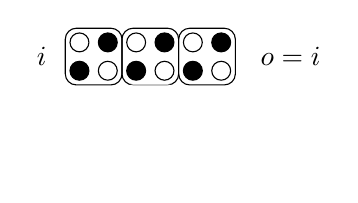
\begin{tikzpicture}
			%One QCA-Cell
			\node (I2) at (-0.3,0.36) {$i$};
			\draw[rounded corners] (0, 0) rectangle (1.2*0.6, 1.2*0.6) [label=north:$v_7$]{};
			
			\draw [fill = black](0.3*0.6,0.3*0.6) circle (2*0.6mm);
			\draw (0.9*0.6,0.3*0.6) circle (2*0.6mm);
			\draw (0.3*0.6,0.9*0.6) circle (2*0.6mm);
			\draw [fill = black](0.9*0.6,0.9*0.6) circle (2*0.6mm);
			
			
			%One QCA-Cell
			\def\x{0.72}
			\draw[rounded corners] (\x, 0) rectangle (1.2*0.6 + \x, 1.2*0.6) {};
			
			\draw [fill = black] (0.3*0.6+\x,0.3*0.6) circle (2*0.6mm);
			\draw (0.9*0.6+\x,0.3*0.6) circle (2*0.6mm);
			\draw (0.3*0.6+\x,0.9*0.6) circle (2*0.6mm);
			\draw [fill = black] (0.9*0.6+\x,0.9*0.6) circle (2*0.6mm);
			
			%One QCA-Cell
%			\def\o{0.72}
%			\def\x{0.72}
%			\draw[rounded corners] (\x, 0 + \o) rectangle (1.2*0.6 + \x, 1.2*0.6 +\o) {};
%			\draw (0.3*0.6+\x,0.3*0.6+\o) circle (2*0.6mm);
%			\draw [fill = black](0.9*0.6+\x,0.3*0.6+\o) circle (2*0.6mm);
%			\draw [fill = black](0.3*0.6+\x,0.9*0.6+\o) circle (2*0.6mm);
%			\draw (0.9*0.6+\x,0.9*0.6+\o) circle (2*0.6mm);
%			\node (I2) at (0.36 + \x,1.7) {$i_1$};
			
			
			%One QCA-Cell
			\def\o{-0.72}
			\def\x{0.72}
			\draw[rounded corners, draw=white] (\x, 0 + \o) rectangle (1.2*0.6 + \x, 1.2*0.6 +\o) {};
%			\draw (0.3*0.6+\x,0.3*0.6+\o) circle (2*0.6mm);
%			\draw [fill = black](0.9*0.6+\x,0.3*0.6+\o) circle (2*0.6mm);
%			\draw [fill = black](0.3*0.6+\x,0.9*0.6+\o) circle (2*0.6mm);
%			\draw (0.9*0.6+\x,0.9*0.6+\o) circle (2*0.6mm);
			\node(I2) at (0.36 + \x,-1.02) {};
			
			%One QCA-Cell
			\def\x{1.44}
			\draw[rounded corners] (\x, 0) rectangle (1.2*0.6 + \x, 1.2*0.6) {};
			
			\draw [fill = black] (0.3*0.6+\x,0.3*0.6) circle (2*0.6mm);
			\draw (0.9*0.6+\x,0.3*0.6) circle (2*0.6mm);
			\draw (0.3*0.6+\x,0.9*0.6) circle (2*0.6mm);
			\draw [fill = black] (0.9*0.6+\x,0.9*0.6) circle (2*0.6mm);
			
			\node (C1) at (0.72 + \x + 0.7, 0.36) {$o = i$};
		\end{tikzpicture} 
		\label{subfig:straight_wire}
	}
\subfigure[Bent wire]
{
	\centering
	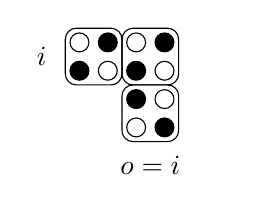
\begin{tikzpicture}
		%One QCA-Cell
		\node (I2) at (-0.3,0.36) {$i$};
		\draw[rounded corners] (0, 0) rectangle (1.2*0.6, 1.2*0.6) [label=north:$v_7$]{};
		
		\draw [fill = black](0.3*0.6,0.3*0.6) circle (2*0.6mm);
		\draw (0.9*0.6,0.3*0.6) circle (2*0.6mm);
		\draw (0.3*0.6,0.9*0.6) circle (2*0.6mm);
		\draw [fill = black](0.9*0.6,0.9*0.6) circle (2*0.6mm);
		
		
		%One QCA-Cell
		\def\x{0.72}
		\draw[rounded corners] (\x, 0) rectangle (1.2*0.6 + \x, 1.2*0.6) {};
		
		\draw [fill = black] (0.3*0.6+\x,0.3*0.6) circle (2*0.6mm);
		\draw (0.9*0.6+\x,0.3*0.6) circle (2*0.6mm);
		\draw (0.3*0.6+\x,0.9*0.6) circle (2*0.6mm);
		\draw [fill = black] (0.9*0.6+\x,0.9*0.6) circle (2*0.6mm);
		
		%One QCA-Cell
%		\def\o{0.72}
%		\def\x{0.72}
%		\draw[rounded corners] (\x, 0 + \o) rectangle (1.2*0.6 + \x, 1.2*0.6 +\o) {};
%		\draw (0.3*0.6+\x,0.3*0.6+\o) circle (2*0.6mm);
%		\draw [fill = black](0.9*0.6+\x,0.3*0.6+\o) circle (2*0.6mm);
%		\draw [fill = black](0.3*0.6+\x,0.9*0.6+\o) circle (2*0.6mm);
%		\draw (0.9*0.6+\x,0.9*0.6+\o) circle (2*0.6mm);
%		\node (I2) at (0.36 + \x,1.7) {$i_1$};
		
		
		%One QCA-Cell
		\def\o{-0.72}
		\def\x{0.72}
		\draw[rounded corners] (\x, 0 + \o) rectangle (1.2*0.6 + \x, 1.2*0.6 +\o) {};
		\draw (0.3*0.6+\x,0.3*0.6+\o) circle (2*0.6mm);
		\draw [fill = black](0.9*0.6+\x,0.3*0.6+\o) circle (2*0.6mm);
		\draw [fill = black](0.3*0.6+\x,0.9*0.6+\o) circle (2*0.6mm);
		\draw (0.9*0.6+\x,0.9*0.6+\o) circle (2*0.6mm);
		\node (I2) at (0.36 + \x,-1.02) {$o=i$};
		
		
		\node (C1) at (0.72 + \x + 0.7, 0.36) {};
	\end{tikzpicture} 
	\label{subfig:bent_wire}
}
\subfigure[Fan-out wire]
{
	\centering
	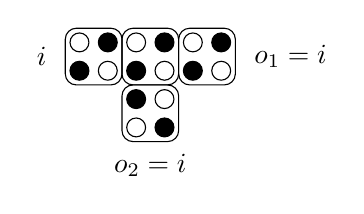
\begin{tikzpicture}
		%One QCA-Cell
		\node (I2) at (-0.3,0.36) {$i$};
		\draw[rounded corners] (0, 0) rectangle (1.2*0.6, 1.2*0.6) [label=north:$v_7$]{};
		
		\draw [fill = black](0.3*0.6,0.3*0.6) circle (2*0.6mm);
		\draw (0.9*0.6,0.3*0.6) circle (2*0.6mm);
		\draw (0.3*0.6,0.9*0.6) circle (2*0.6mm);
		\draw [fill = black](0.9*0.6,0.9*0.6) circle (2*0.6mm);
		
		
		%One QCA-Cell
		\def\x{0.72}
		\draw[rounded corners] (\x, 0) rectangle (1.2*0.6 + \x, 1.2*0.6) {};
		
		\draw [fill = black] (0.3*0.6+\x,0.3*0.6) circle (2*0.6mm);
		\draw (0.9*0.6+\x,0.3*0.6) circle (2*0.6mm);
		\draw (0.3*0.6+\x,0.9*0.6) circle (2*0.6mm);
		\draw [fill = black] (0.9*0.6+\x,0.9*0.6) circle (2*0.6mm);
		
		%One QCA-Cell
%		\def\o{0.72}
%		\def\x{0.72}
%		\draw[rounded corners] (\x, 0 + \o) rectangle (1.2*0.6 + \x, 1.2*0.6 +\o) {};
%		\draw (0.3*0.6+\x,0.3*0.6+\o) circle (2*0.6mm);
%		\draw [fill = black](0.9*0.6+\x,0.3*0.6+\o) circle (2*0.6mm);
%		\draw [fill = black](0.3*0.6+\x,0.9*0.6+\o) circle (2*0.6mm);
%		\draw (0.9*0.6+\x,0.9*0.6+\o) circle (2*0.6mm);
%		\node (I2) at (0.36 + \x,1.7) {$i_1$};
		
		
		%One QCA-Cell
		\def\o{-0.72}
		\def\x{0.72}
		\draw[rounded corners] (\x, 0 + \o) rectangle (1.2*0.6 + \x, 1.2*0.6 +\o) {};
		\draw (0.3*0.6+\x,0.3*0.6+\o) circle (2*0.6mm);
		\draw [fill = black](0.9*0.6+\x,0.3*0.6+\o) circle (2*0.6mm);
		\draw [fill = black](0.3*0.6+\x,0.9*0.6+\o) circle (2*0.6mm);
		\draw (0.9*0.6+\x,0.9*0.6+\o) circle (2*0.6mm);
		\node (I2) at (0.36 + \x,-1.02) {$o_2 = i$};
		
		%One QCA-Cell
		\def\x{1.44}
		\draw[rounded corners] (\x, 0) rectangle (1.2*0.6 + \x, 1.2*0.6) {};
		
		\draw [fill = black] (0.3*0.6+\x,0.3*0.6) circle (2*0.6mm);
		\draw (0.9*0.6+\x,0.3*0.6) circle (2*0.6mm);
		\draw (0.3*0.6+\x,0.9*0.6) circle (2*0.6mm);
		\draw [fill = black] (0.9*0.6+\x,0.9*0.6) circle (2*0.6mm);
		
		\node (C1) at (0.72 + \x + 0.7, 0.36) {$o_1 = i$};
	\end{tikzpicture} 
	\label{subfig:fanout_wire}
}

	\caption{QCA wires}\label{fig:QCA_wires}
\end{figure}

Unlike in CMOS technology, in QCA, wires must also be treated as gates. As previously demonstrated in Figure~\ref{fig:QCAWire}, a QCA wire also comprises of QCA cells and thus can be treated as a gate. Since wires do not add any additional functionality to the logic, they are considered to represent the identity function. This property has the significant drawback of the cost of wires being comparable to that of other logic gates, which is often used as a major cost metric in circuit design. Until now, only straight planar wires have been considered. From the implementation of the majority gate, it is already evident that data is not only transferred in the x-dimension but also in the y-dimension, requiring the wiring to also be able to flow in both dimensions. When gates are placed side-by-side in two dimensions, the resulting circuit can be viewed as a 2D-grid. To allow information to change its propagation direction from the x-direction to the y-direction and vice versa, bent wires must also be introduced. They are depicted in Figure~\ref{subfig:bent_wire} and show a 90-degree bend. Since all tiles can be rotated by $90^{\circ}$, $180^{\circ}$ and $270^{\circ}$ respectively, a tile connected to a bent wire can be routed to each adjacent tile of a bent wire. Additionally, since all gates introduced so far have a fan-out of one, we need a fan-out node to duplicate signals. This is achieved by adding a bent wire to a straight wire, resulting in the fan-out shown in Figure~\ref{subfig:fanout_wire}.
%%%%Wire crossing
\begin{figure}
	\centering
	\subfigure[Coplanar wire crossing]
	{
		\centering
		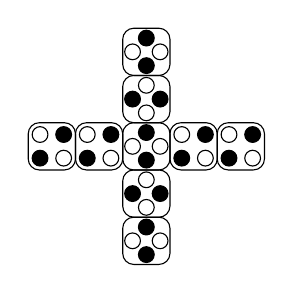
\begin{tikzpicture}
			%One QCA-Cell
			%\node (I2) at (-0.3,0.36) {$i$};
			\draw[rounded corners] (0, 0) rectangle (1.2*0.5, 1.2*0.5) [label=north:$v_7$]{};
			
			\draw [fill = black](0.3*0.5,0.3*0.5) circle (2*0.5mm);
			\draw (0.9*0.5,0.3*0.5) circle (2*0.5mm);
			\draw (0.3*0.5,0.9*0.5) circle (2*0.5mm);
			\draw [fill = black](0.9*0.5,0.9*0.5) circle (2*0.5mm);
			
			
			%One QCA-Cell
			\def\x{0.6}
			\draw[rounded corners] (\x, 0) rectangle (1.2*0.5 + \x, 1.2*0.5) {};
			
			\draw [fill = black] (0.3*0.5+\x,0.3*0.5) circle (2*0.5mm);
			\draw (0.9*0.5+\x,0.3*0.5) circle (2*0.5mm);
			\draw (0.3*0.5+\x,0.9*0.5) circle (2*0.5mm);
			\draw [fill = black] (0.9*0.5+\x,0.9*0.5) circle (2*0.5mm);
			
			%One QCA-Cell
			\def\o{0}
			\def\x{1.2}
			\draw[rounded corners] (\x, 0 + \o) rectangle (1.2*0.5 + \x, 1.2*0.5 +\o) {};
			\draw [fill = black](0.6*0.5+\x,0.3*0.5+\o - 0.025) circle (2*0.5mm);
			\draw (0.9*0.5+\x + 0.025,0.6*0.5+\o) circle (2*0.5mm);
			\draw (0.3*0.5+\x - 0.025,0.6*0.5+\o) circle (2*0.5mm);
			\draw [fill = black](0.6*0.5+\x,0.9*0.5+\o + 0.025) circle (2*0.5mm);
			
			%One QCA-Cell
			\def\x{1.8}
			\draw[rounded corners] (\x, 0) rectangle (1.2*0.5 + \x, 1.2*0.5) {};
			
			\draw [fill = black] (0.3*0.5+\x,0.3*0.5) circle (2*0.5mm);
			\draw (0.9*0.5+\x,0.3*0.5) circle (2*0.5mm);
			\draw (0.3*0.5+\x,0.9*0.5) circle (2*0.5mm);
			\draw [fill = black] (0.9*0.5+\x,0.9*0.5) circle (2*0.5mm);
			
			%One QCA-Cell
			\def\x{2.4}
			\draw[rounded corners] (\x, 0) rectangle (1.2*0.5 + \x, 1.2*0.5) {};
			
			\draw [fill = black] (0.3*0.5+\x,0.3*0.5) circle (2*0.5mm);
			\draw (0.9*0.5+\x,0.3*0.5) circle (2*0.5mm);
			\draw (0.3*0.5+\x,0.9*0.5) circle (2*0.5mm);
			\draw [fill = black] (0.9*0.5+\x,0.9*0.5) circle (2*0.5mm);
			
			%One QCA-Cell
			\def\o{0.6}
			\def\x{1.2}
			\draw[rounded corners] (\x, 0 + \o) rectangle (1.2*0.5 + \x, 1.2*0.5 +\o) {};
			\draw (0.6*0.5+\x,0.3*0.5+\o - 0.025) circle (2*0.5mm);
			\draw [fill = black](0.9*0.5+\x + 0.025,0.6*0.5+\o) circle (2*0.5mm);
			\draw [fill = black](0.3*0.5+\x - 0.025,0.6*0.5+\o) circle (2*0.5mm);
			\draw (0.6*0.5+\x,0.9*0.5+\o + 0.025) circle (2*0.5mm);
			
			%One QCA-Cell
			\def\o{1.2}
			\def\x{1.2}
			\draw[rounded corners] (\x, 0 + \o) rectangle (1.2*0.5 + \x, 1.2*0.5 +\o) {};
			\draw [fill = black](0.6*0.5+\x,0.3*0.5+\o - 0.025) circle (2*0.5mm);
			\draw (0.9*0.5+\x + 0.025,0.6*0.5+\o) circle (2*0.5mm);
			\draw (0.3*0.5+\x - 0.025,0.6*0.5+\o) circle (2*0.5mm);
			\draw [fill = black](0.6*0.5+\x,0.9*0.5+\o + 0.025) circle (2*0.5mm);
			
			%One QCA-Cell
			\def\o{-0.6}
			\def\x{1.2}
			\draw[rounded corners] (\x, 0 + \o) rectangle (1.2*0.5 + \x, 1.2*0.5 +\o) {};
			\draw (0.6*0.5+\x,0.3*0.5+\o - 0.025) circle (2*0.5mm);
			\draw [fill = black](0.9*0.5+\x + 0.025,0.6*0.5+\o) circle (2*0.5mm);
			\draw [fill = black](0.3*0.5+\x - 0.025,0.6*0.5+\o) circle (2*0.5mm);
			\draw (0.6*0.5+\x,0.9*0.5+\o + 0.025) circle (2*0.5mm);
			
			%One QCA-Cell
			\def\o{-1.2}
			\def\x{1.2}
			\draw[rounded corners] (\x, 0 + \o) rectangle (1.2*0.5 + \x, 1.2*0.5 +\o) {};
			\draw [fill = black](0.6*0.5+\x,0.3*0.5+\o - 0.025) circle (2*0.5mm);
			\draw (0.9*0.5+\x + 0.025,0.6*0.5+\o) circle (2*0.5mm);
			\draw (0.3*0.5+\x - 0.025,0.6*0.5+\o) circle (2*0.5mm);
			\draw [fill = black](0.6*0.5+\x,0.9*0.5+\o + 0.025) circle (2*0.5mm);
		\end{tikzpicture} 
		\label{subfig:CoplanarWire}
	}
	\subfigure[Multi-layer wire crossing]
	{
		\centering
		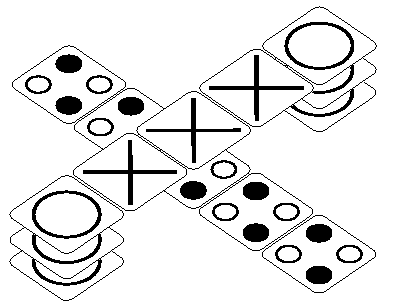
\includegraphics[scale=0.55]{ML_WC}
		\label{subfig:mlwirecrossing}
	}
	
	\caption{Different QCA wire crossing implementations} 
\end{figure}

The last special case of wires is the crossing case. By rotating the cells of one wire string by $45^{\circ}$, the rotated cells do not couple with non-rotated cells \cite{Inverter_displacements}, as shown in Figure~\ref{subfig:CoplanarWire}. This solution is very useful because it supports the planar structure of the circuit and is therefore referred to as \textit{coplanar wire crossing}. Additionally, the possibility of multi-layer QCA has been investigated \cite{multi_lyer_wire_crossing} and found to be particularly useful in the case of wire crossings. To achieve this, one wire string is raised to an additional higher layer, which is connected with a vertical interconnect, as shown in Figure~\ref{subfig:mlwirecrossing}. The signal transmission in the vertically-stacked cells works in the same way as in the horizontal direction. To prevent any crosstalk between the wire strings, intermediate layers of cells are used in the vertical direction. Theoretically, the top layer can not only be used as a wire, but since the signal distribution works in the same way as in the ground layer, gates can also be placed in these multi-layers. Simulations have shown that coplanar crossovers significantly reduce the coupling between the horizontal wire segments, making the horizontal interconnect very sensitive to crosstalk and therefore highly prone to cell displacements \cite{Inverter_displacements}. Multilayer circuits, on the other hand, show high robustness and are therefore used as a standard in this library. In the tile representation of the multilayer interconnect, the top wire string is represented with a $\times$, while the vertical layers are represented with a circle. It should be noted that the complex structure of the multilayer wire crossing yields high costs and is therefore avoided in the design of QCA circuits. In Figure~\ref{fig:StandardCellLibrary}, all gates used in this work are summarized.

\begin{figure}
	\centering
	\subfigure[INV]
	{
		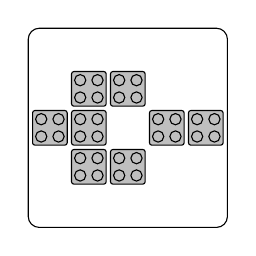
\begin{tikzpicture}[rotate=90, scale=1.1, every node/.style={scale=1.2}]
			\draw[rounded corners] (-0.05, -0.1 - 0.85) rectangle (2.3-0.05, 2.3-0.1 - 0.85){};
			
			\foreach \x/\y in {0.9/0.9, 0.9/0.45, 1.35/0.45, 0.45/0.45, 1.35/0, 0.45/0, 0.9/-0.45, 0.9/-0.9}
			{
				\draw[rounded corners = 0.3mm, fill=lightgray] (\x, 0 + \y) rectangle (1.2/3 + \x, 1.2/3 + \y){};
				\draw (0.3/3+ \x,0.3/3 + \y) circle (0.65mm);
				\draw (0.9/3+ \x,0.3/3+ \y) circle (0.65mm);
				\draw (0.3/3+ \x,0.9/3 + \y) circle (0.65mm);
				\draw (0.9/3+ \x,0.9/3 + \y) circle (0.65mm);
			}
		\end{tikzpicture}
	}
\subfigure[MAJ]
{
	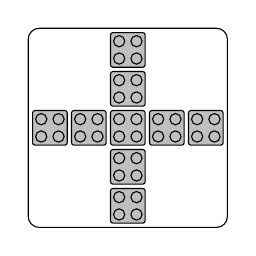
\begin{tikzpicture}[rotate=90, scale=1.1, every node/.style={scale=1.2}]
		\draw[rounded corners] (-0.05, -0.1 - 0.85) rectangle (2.3-0.05, 2.3-0.1 - 0.85){};
		
		\foreach \x/\y in {0.9/0.9, 0.9/0.45, 0.9/0, 0.9/-0.45, 0.9/-0.9, 0/0, 0.45/0, 1.35/0, 1.8/0}
		{
			\draw[rounded corners = 0.3mm, fill=lightgray] (\x, 0 + \y) rectangle (1.2/3 + \x, 1.2/3 + \y){};
			\draw (0.3/3+ \x,0.3/3 + \y) circle (0.65mm);
			\draw (0.9/3+ \x,0.3/3+ \y) circle (0.65mm);
			\draw (0.3/3+ \x,0.9/3 + \y) circle (0.65mm);
			\draw (0.9/3+ \x,0.9/3 + \y) circle (0.65mm);
		}
	\end{tikzpicture}
}
\subfigure[AND]
{
	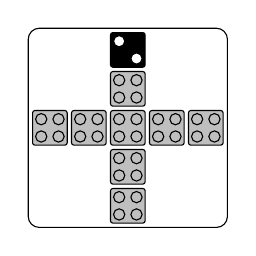
\begin{tikzpicture}[rotate=90, scale=1.1, every node/.style={scale=1.2}]
		\draw[rounded corners] (-0.05, -0.1 - 0.85) rectangle (2.3-0.05, 2.3-0.1 - 0.85){};
		
		\foreach \x/\y in {0.9/0.9, 0.9/0.45, 0.9/0, 0.9/-0.45, 0.9/-0.9, 0/0, 0.45/0, 1.35/0}
		{
			\draw[rounded corners = 0.3mm, fill=lightgray] (\x, 0 + \y) rectangle (1.2/3 + \x, 1.2/3 + \y){};
			\draw (0.3/3+ \x,0.3/3 + \y) circle (0.65mm);
			\draw (0.9/3+ \x,0.3/3+ \y) circle (0.65mm);
			\draw (0.3/3+ \x,0.9/3 + \y) circle (0.65mm);
			\draw (0.9/3+ \x,0.9/3 + \y) circle (0.65mm);
		}
		\foreach \x/\y in {1.8/0}
		{
			\draw[rounded corners = 0.3mm, fill=black] (\x, 0 + \y) rectangle 	(1.2/3 + \x, 1.2/3 + \y){};
			\draw [fill=white](0.3/3+ \x,0.3/3 + \y) circle (0.65mm);
			\draw (0.9/3+ \x,0.3/3+ \y) circle (0.65mm);
			\draw (0.3/3+ \x,0.9/3 + \y) circle (0.65mm);
			\draw [fill=white](0.9/3+ \x,0.9/3 + \y) circle (0.65mm);
		}
	\end{tikzpicture}
}
\subfigure[OR]
{
	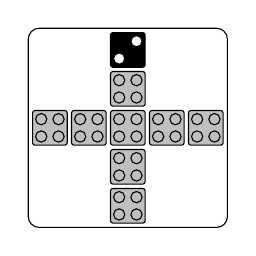
\begin{tikzpicture}[rotate=90, scale=1.1, every node/.style={scale=1.2}]
		\draw[rounded corners] (-0.05, -0.1 - 0.85) rectangle (2.3-0.05, 2.3-0.1 - 0.85){};
		
		\foreach \x/\y in {0.9/0.9, 0.9/0.45, 0.9/0, 0.9/-0.45, 0.9/-0.9, 0/0, 0.45/0, 1.35/0}
		{
			\draw[rounded corners = 0.3mm, fill=lightgray] (\x, 0 + \y) rectangle (1.2/3 + \x, 1.2/3 + \y){};
			\draw (0.3/3+ \x,0.3/3 + \y) circle (0.65mm);
			\draw (0.9/3+ \x,0.3/3+ \y) circle (0.65mm);
			\draw (0.3/3+ \x,0.9/3 + \y) circle (0.65mm);
			\draw (0.9/3+ \x,0.9/3 + \y) circle (0.65mm);
		}
		\foreach \x/\y in {1.8/0}
		{
			\draw[rounded corners = 0.3mm, fill=black] (\x, 0 + \y) rectangle 	(1.2/3 + \x, 1.2/3 + \y){};
			\draw (0.3/3+ \x,0.3/3 + \y) circle (0.65mm);
			\draw [fill=white](0.9/3+ \x,0.3/3+ \y) circle (0.65mm);
			\draw [fill=white](0.3/3+ \x,0.9/3 + \y) circle (0.65mm);
			\draw (0.9/3+ \x,0.9/3 + \y) circle (0.65mm);
		}
	\end{tikzpicture}
}\\
\subfigure[Wire]
{
	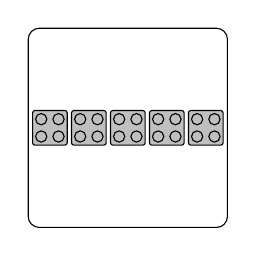
\begin{tikzpicture}[rotate=90, scale=1.1, every node/.style={scale=1.2}]
		\draw[rounded corners] (-0.05, -0.1 - 0.85) rectangle (2.3-0.05, 2.3-0.1 - 0.85){};
		
		\foreach \x/\y in {0.9/0.9, 0.9/0.45, 0.9/0, 0.9/-0.45, 0.9/-0.9}
		{
			\draw[rounded corners = 0.3mm, fill=lightgray] (\x, 0 + \y) rectangle (1.2/3 + \x, 1.2/3 + \y){};
			\draw (0.3/3+ \x,0.3/3 + \y) circle (0.65mm);
			\draw (0.9/3+ \x,0.3/3+ \y) circle (0.65mm);
			\draw (0.3/3+ \x,0.9/3 + \y) circle (0.65mm);
			\draw (0.9/3+ \x,0.9/3 + \y) circle (0.65mm);
		}
	\end{tikzpicture}
}
\subfigure[Bent wire]
{
	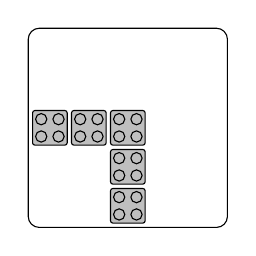
\begin{tikzpicture}[rotate=90, scale=1.1, every node/.style={scale=1.2}]
		\draw[rounded corners] (-0.05, -0.1 - 0.85) rectangle (2.3-0.05, 2.3-0.1 - 0.85){};
		
		\foreach \x/\y in {0.9/0.9, 0.9/0.45, 0.9/0, 0/0, 0.45/0}
		{
			\draw[rounded corners = 0.3mm, fill=lightgray] (\x, 0 + \y) rectangle (1.2/3 + \x, 1.2/3 + \y){};
			\draw (0.3/3+ \x,0.3/3 + \y) circle (0.65mm);
			\draw (0.9/3+ \x,0.3/3+ \y) circle (0.65mm);
			\draw (0.3/3+ \x,0.9/3 + \y) circle (0.65mm);
			\draw (0.9/3+ \x,0.9/3 + \y) circle (0.65mm);
		}
	\end{tikzpicture}
	\label{subfig:BentWire}
}
\subfigure[Fanout]
{
	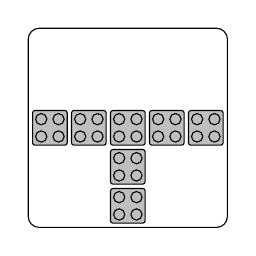
\begin{tikzpicture}[rotate=90, scale=1.1, every node/.style={scale=1.2}]
		\draw[rounded corners] (-0.05, -0.1 - 0.85) rectangle (2.3-0.05, 2.3-0.1 - 0.85){};
		
		\foreach \x/\y in {0.9/0.9, 0.9/0.45, 0.9/0, 0.9/-0.45, 0.9/-0.9, 0/0, 0.45/0}
		{
			\draw[rounded corners = 0.3mm, fill=lightgray] (\x, 0 + \y) rectangle (1.2/3 + \x, 1.2/3 + \y){};
			\draw (0.3/3+ \x,0.3/3 + \y) circle (0.65mm);
			\draw (0.9/3+ \x,0.3/3+ \y) circle (0.65mm);
			\draw (0.3/3+ \x,0.9/3 + \y) circle (0.65mm);
			\draw (0.9/3+ \x,0.9/3 + \y) circle (0.65mm);
		}
	\end{tikzpicture}
	\label{subfig:FanoutWire}
}
\subfigure[Wire crossing]
{
	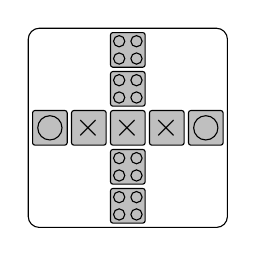
\begin{tikzpicture}[rotate=90, scale=1.1, every node/.style={scale=1.2}]
		\draw[rounded corners] (-0.05, -0.1 - 0.85) rectangle (2.3-0.05, 2.3-0.1 - 0.85){};
		
		\foreach \x/\y in {0/0, 0.45/0, 1.35/0, 1.8/0}
		{
			\draw[rounded corners = 0.3mm, fill=lightgray] (\x, 0 + \y) rectangle (1.2/3 + \x, 1.2/3 + \y){};
			\draw (0.3/3+ \x,0.3/3 + \y) circle (0.65mm);
			\draw (0.9/3+ \x,0.3/3+ \y) circle (0.65mm);
			\draw (0.3/3+ \x,0.9/3 + \y) circle (0.65mm);
			\draw (0.9/3+ \x,0.9/3 + \y) circle (0.65mm);
		}
		\foreach \x/\y in {0.9/-0.45, 0.9/0, 0.9/0.45}
		{
			\draw[rounded corners = 0.3mm, fill=lightgray] (\x, 0 + \y) rectangle 	(1.2/3 + \x, 1.2/3 + \y){};
			\node (X) at (\x + 0.5*0.45- 0.025, \y + 0.5*0.45 - 0.025) {$\times$};
			
		}
		\foreach \x/\y in {0.9/-0.9, 0.9/0.9}
		{
			\draw[rounded corners = 0.3mm, fill=lightgray] (\x, 0 + \y) rectangle (1.2/3 + \x, 1.2/3 + \y){};
			\draw (\x + 0.5*0.45- 0.025, \y + 0.5*0.45 - 0.025) circle (1.4mm){};
			
		}
	\end{tikzpicture}
}
	\caption{QCA Standard Library}\label{fig:StandardCellLibrary}
\end{figure}

\subsection{Clocking}\label{subsec:clocking}

As mentioned above, data transfer in the QCA paradigm is accomplished by cell-to-cell interaction. Given a fixed polarization of a cell, the next cell reacts to the Coulomb repulsion and changes its polarization accordingly. Looking back at the wire segment in Figure~\ref{fig:QCAWire}, the leftmost cell has a fixed polarization and is called the input. After some time the information propagates through to the rightmost cell, representing the output of the simplified QCA-circuit. Generally, a QCA circuit can be seen as an assembly of cells on a two-dimensional grid or array, where each cell has a position with $x$ and $y$ coordinates assigned. Every cell with fixed polarization is called an input cell and drives the other cells gradually into matching polarization. When all cells have matching polarization, meaning that the electrons in two adjacent cells have the maximum distance and therefore minimum energy following Coulomb repulsion, the QCA array is said to be in \emph{ground state} \cite{lent1997device}. When a cell does not contribute to the signal propagation of the circuit, it is called an output cell. While the polarization is propagating through the array, the direction of the propagation is always pointing away from the input cells and to the output cells. In reality the propagation doesn't go gradually through the array but shows a quite unpredictable behavior~\cite{lent1994quantum}. This is the first reason, why a \textit{clocking}, involving well-defined states for the polarization of the cells and enabling a well-ordered signal propagation, was introduced. Another reason for a clocking is, that for the described straight forward process called \emph{abrupt switching}~\cite{lent1997device} with dissipative coupling to the environment, the QCA-array has to be embedded into a CMOS environment, as shown in Figure~\ref{fig:QCA_array}. In the following, a short evolution of this primitive clocking to the currently used clocking is described.

\begin{figure}
	\centering
	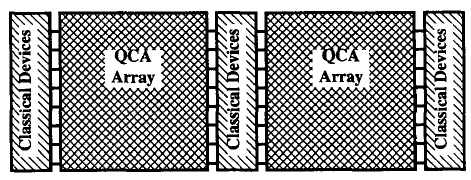
\includegraphics[scale=0.6]{QCA_array}
	\caption{Schematic of a combined QCA and CMOS system \cite{lent1994quantum}.} 
	\label{fig:QCA_array}
\end{figure}

Therefore, the QCA-Array is divided into smaller decoupled sub-regions called \emph{clock zones} and each clock zone receives an external signal, a clock, assigned \cite{lent1997device}. The clock can then activate and deactivate the cells of a zone in a way that the information propagates gradually from one zone to the next through the whole QCA circuit. In the approach first used, the clock decreases the QD barriers of all cells in a clock zone, when applying a new input. This means that the electrons are not trapped and can move freely following Coulomb repulsion, therefore taking over the polarization of the input cell. When all cells in the region are stable, the barriers are raised again, localizing the electrons in the cells, which now have the desired polarization. Meanwhile, the barriers of the subsequent clock zone are lowered simultaneously, the previous sub-region acts as fixed input and again the polarization is taken over. In this way, the information gradually propagates through the whole circuit~\cite{lent1997device}. Today's used approaches create electrical fields with an external clock generator and distribute it to the cells through the device substrate using embedded electrodes. Thereby, the energy level of the \textit{null} state can be controlled, resulting in an equivalent effect as in the former approach~\cite{Walter}.

\begin{figure}
	\centering
	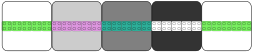
\includegraphics[scale=0.41]{clocked_wire}
	\caption{QCA wire divided into the four clock zones according to Bennett clocking}\label{fig:QCA_wire_clocked}
\end{figure}

A wire divided into clock zones is shown in Figure~\ref{fig:QCA_wire_clocked}. The colors of the zones and cells, as well as the zone number, provide redundant information about the type of clock zone. They differ in the external applied electrical field and, therefore, the energy of the cells. In QCA, the clocking is divided into four consecutive states: \emph{switch}, \emph{hold}, \emph{release}, and \emph{relax}. They are aligned in a pipeline-like structure, where each of these states is phase-shifted by $\frac{\pi}{2}$, forming a $2\pi$ clock cycle. In the switch phase, cells start to get polarized, depending on the polarization of the driving cell. When the cells are polarized, they get fixed in the hold-phase. Afterwards, in the release-phase, the excitation gradually decreases, resulting in the unexcited relax-state \cite{Sasamal2020QuantumDotCA}. After one clocking cycle, the next clocking cycle starts with the same order of states, also denoted with numbers $i = {1, 2, 3, 4}$. Hence, for consecutive clocking numbers $(i_{next} = i_{previous}+1 \mod clk)$ holds. The scheme of such a pipeline as clocking is depicted exemplary in Figure~\ref{subfig:Landauer}.

%%%%%%%%%%%%%%%%%%%%%%%%%%%%%%%%%%%%%%%%%%%%%%%%%%%%%%%%%%%%%

\begin{figure}
	\centering
	\subfigure[Landauer clocking]{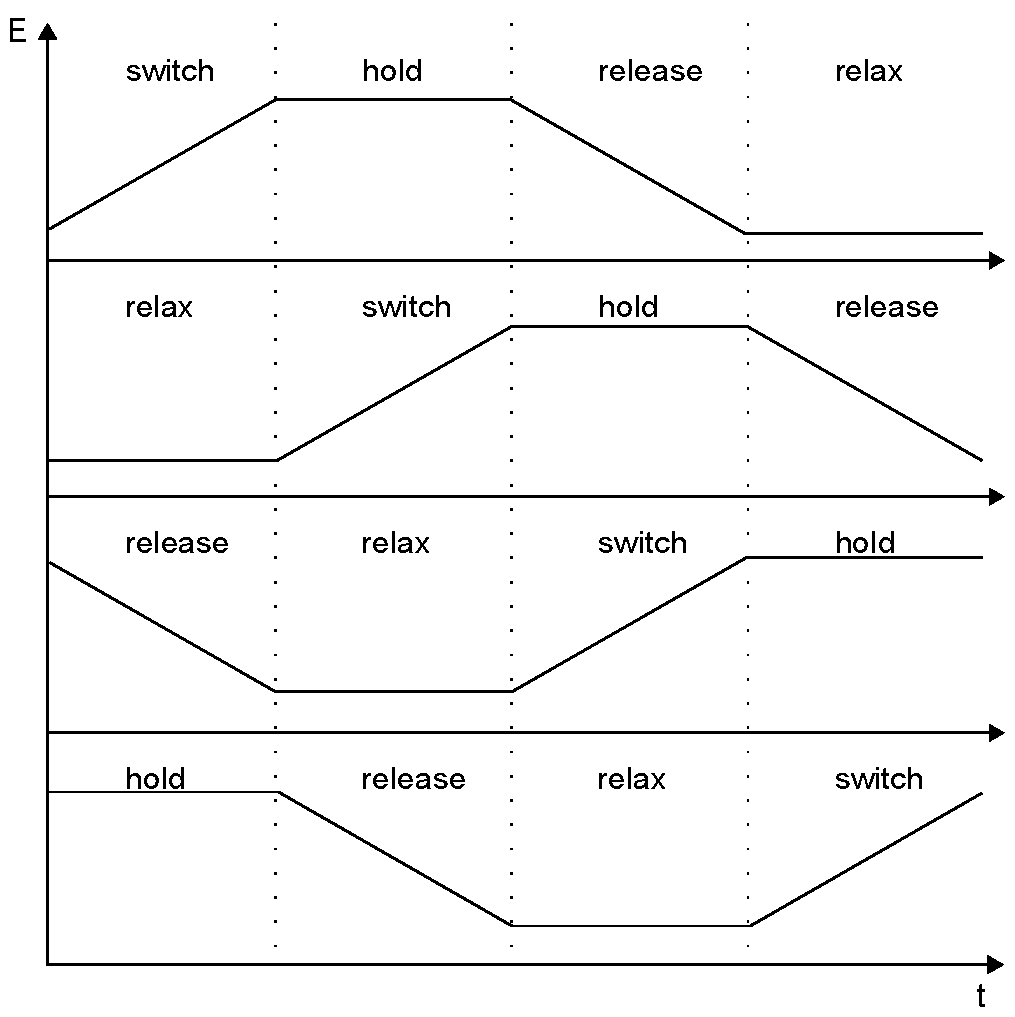
\includegraphics[scale=0.41]{Landauer_clocking}\label{subfig:Landauer}}
	\subfigure[Bennet clocking]{\includegraphics[scale=0.41]{Bennet_clocking}\label{subfig:Bennet}}
	\caption{QCA clocking pipeline} \label{fig:QCAClockpipeline}
\end{figure}


The described clocking is known as \textit{Landauer clocking}~\cite{lent1997device}. Its name giver, Rolf Landauer, pointed out the significant power dissipation of this clocking mechanism. The main cause of high power dissipation is the \textit{erase} function, which occurs because in Landauer clocking the release state directly follows the hold phase, irreversibly erasing the information and, therefore, transforming it into heat~\cite{landauer1961irreversibility}. To address this issue in the QCA domain, Landauer proposed that the erase function must be eliminated from the clocking. He argued that every erased bit dissipates at least $k_BT\ln(2)$ in heat dissipation~\cite{keyes1970minimal}. For example, if a QCA-cell has a size of $1nm \times 1nm$ and an operating frequency of $100 GHz$, the corresponding density of devices results in $10^{14}$ $cm^{-2}$. Additionally, if a dissipation of $0.1 eV$ every clock cycle is assumed, it results in a total power dissipation of $160 kW cm^{-2}$. This directly implies that a device operating with this clocking would be inoperable (it would evaporate due to heat)~\cite{lent2006bennett}. The \textit{Bennett clocking}~\cite{lent2006bennett} tackles exactly this problem by altering the timing of the clocking signals. Just as in the Landauer clocking, the clocking wave propagates in one direction, but leaving no trailing edge, when information is passed. Instead, the cells will be held in the excited state until the information propagates through the whole QCA-array. When the output is read, the excitation is released in reverse order resulting in no erase functions. This means, that this \textit{quasi-adiabatic} clocking leads to a minimal power dissipation but with two constraints: (1) The effective clock rate is at least halved due to the additional backwards propagation and (2) since only one signal vector can be transmitted through the system, the pipeline capabilities are reduced \cite{lent2006bennett}. The resulting clocking scheme for Bennett clocking is shown in Figure~\ref{subfig:Bennet}. In order to preserve the pipeline like behavior of the Landauer clocking and the energetic advantages of the Bennett clocking, QCA circuits are divided into sub-regions, which are each Bennett clocked.

\begin{figure}
	\centering
	\includegraphics[scale=0.9]{cell_MUX}
	\caption{Cell based layout of a 2:1 MUX \cite{majeed2019optimal}}\label{fig:cell_based_mux}
\end{figure}

As already stated, the QCA-array has to be divided into clock zones, in order to apply a proper clocking. Allowing an arbitrary number of cells in one clock zone gives lots of freedom in designing clock zones with variable geometries. This clocking is referred to as \textit{cell-based} and increases the fabrication process due to its variety in clock zone geometries. Assuming the necessity of a uniform fabrication in order to fabricate circuits with millions of cells, this clocking gets infeasible for large circuits. Since in this scheme single cells can be clocked, also electrodes of the same size must be fabricated, in order to provide a clocking signal to the single-cell region. Since this is also not feasible, this design is obsolete \cite{blair2003architecture}. An example of a cell-based clocking design of a 2:1 multiplexer (MUX) can be seen in Figure~\ref{fig:cell_based_mux}. To achieve uniform clock zones with a possible distribution of clocking signals, the \textit{tile-based} clocking is introduced. The approach of this design is to provide uniform tiles of size $3 \times 3$ or $5 \times 5$. For clocking tiles larger than this, information propagation was suggested to be erroneous, also being an argument against cell-based clocking \cite{taucer2015consequences}.


\begin{figure}
	\newcommand*{\xMin}{0}%
	\newcommand*{\xMax}{4}%
	\newcommand*{\xMaxc}{3}%
	\newcommand*{\yMin}{0}%
	\newcommand*{\yMax}{4}%
	\newcommand*{\yMaxc}{3}%
	\subfigure[2DDWave \cite{2DD}]
	{
		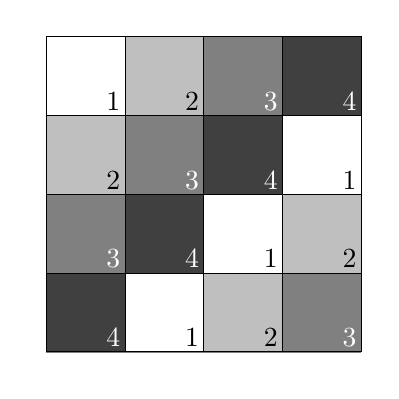
\begin{tikzpicture}
			
			\foreach \i in {\xMin,...,\xMax} {
				\draw [very thin,gray] (\i,\yMin) -- (\i,\yMax)  node [below] at (\i,\yMin) {};
			}
			\foreach \i in {\yMin,...,\yMax} {
				\draw [very thin,gray] (\xMin,\i) -- (\xMax,\i) node [left] at (\xMin,\i) {};
			}
			
			
			\draw[fill=darkgray]  (0, 1) -- (1, 1) -- (1,0) -- (0,0) -- cycle;
			\draw[fill=white]  (1, 1) -- (2, 1) -- (2,0) -- (1,0) -- cycle;
			\draw[fill=lightgray]  (2, 1) -- (3, 1) -- (3,0) -- (2,0) -- cycle;
			\draw[fill=gray]  (3, 1) -- (4, 1) -- (4,0) -- (3,0) -- cycle;
			
			\draw[fill=gray]  (0, 2) -- (1, 2) -- (1,1) -- (0,1) -- cycle;
			\draw[fill=darkgray]  (1, 2) -- (2, 2) -- (2,1) -- (1,1) -- cycle;
			\draw[fill=white]  (2, 2) -- (3, 2) -- (3,1) -- (2,1) -- cycle;
			\draw[fill=lightgray]  (3, 2) -- (4, 2) -- (4,1) -- (3,1) -- cycle;
			
			\draw[fill=lightgray]  (0, 3) -- (1, 3) -- (1,2) -- (0,2) -- cycle;
			\draw[fill=gray]  (1, 3) -- (2, 3) -- (2,2) -- (1,2) -- cycle;
			\draw[fill=darkgray]  (2, 3) -- (3, 3) -- (3,2) -- (2,2) -- cycle;
			\draw[fill=white]  (3, 3) -- (4, 3) -- (4,2) -- (3,2) -- cycle;
			
			\draw[fill=white]  (0, 4) -- (1, 4) -- (1,3) -- (0,3) -- cycle;
			\draw[fill=lightgray]  (1, 4) -- (2, 4) -- (2,3) -- (1,3) -- cycle;
			\draw[fill=gray]  (2, 4) -- (3, 4) -- (3,3) -- (2,3) -- cycle;
			\draw[fill=darkgray]  (3, 4) -- (4, 4) -- (4,3) -- (3,3) -- cycle;
			
			\node[text=white] (A1) at (0.85,0.18) {$4$};
			\node[text=black] (A1) at (1.85,0.18) {$1$};
			\node[text=black] (A1) at (2.85,0.18) {$2$};
			\node[text=white] (A1) at (3.85,0.18) {$3$};
			
			\node[text=white] (A1) at (0.85,1.18) {$3$};
			\node[text=white] (A1) at (1.85,1.18) {$4$};
			\node[text=black] (A1) at (2.85,1.18) {$1$};
			\node[text=black] (A1) at (3.85,1.18) {$2$};
			
			\node[text=black] (A1) at (0.85,2.18) {$2$};
			\node[text=white] (A1) at (1.85,2.18) {$3$};
			\node[text=white] (A1) at (2.85,2.18) {$4$};
			\node[text=black] (A1) at (3.85,2.18) {$1$};
			
			\node[text=black] (A1) at (0.85,3.18) {$1$};
			\node[text=black] (A1) at (1.85,3.18) {$2$};
			\node[text=white] (A1) at (2.85,3.18) {$3$};
			\node[text=white] (A1) at (3.85,3.18) {$4$};
			
			
		\end{tikzpicture}
		\label{subfig:2DD}
	}
	\subfigure[USE \cite{USE}]
	{
		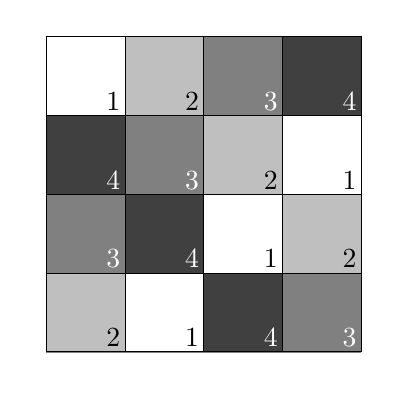
\begin{tikzpicture}
			\foreach \i in {\xMin,...,\xMax} {
				\draw [very thin,gray] (\i,\yMin) -- (\i,\yMax)  node [below] at (\i,\yMin) {};
			}
			\foreach \i in {\yMin,...,\yMax} {
				\draw [very thin,gray] (\xMin,\i) -- (\xMax,\i)
				node [left] at (\xMin,\i) {};
			}
			\draw[fill=lightgray]  (0, 1) -- (1, 1) -- (1,0) -- (0,0) -- cycle;
			\draw[fill=white]  (1, 1) -- (2, 1) -- (2,0) -- (1,0) -- cycle;
			\draw[fill=darkgray]  (2, 1) -- (3, 1) -- (3,0) -- (2,0) -- cycle;
			\draw[fill=gray]  (3, 1) -- (4, 1) -- (4,0) -- (3,0) -- cycle;
			
			\draw[fill=gray]  (0, 2) -- (1, 2) -- (1,1) -- (0,1) -- cycle;
			\draw[fill=darkgray]  (1, 2) -- (2, 2) -- (2,1) -- (1,1) -- cycle;
			\draw[fill=white]  (2, 2) -- (3, 2) -- (3,1) -- (2,1) -- cycle;
			\draw[fill=lightgray]  (3, 2) -- (4, 2) -- (4,1) -- (3,1) -- cycle;
			
			\draw[fill=darkgray]  (0, 3) -- (1, 3) -- (1,2) -- (0,2) -- cycle;
			\draw[fill=gray]  (1, 3) -- (2, 3) -- (2,2) -- (1,2) -- cycle;
			\draw[fill=lightgray]  (2, 3) -- (3, 3) -- (3,2) -- (2,2) -- cycle;
			\draw[fill=white]  (3, 3) -- (4, 3) -- (4,2) -- (3,2) -- cycle;
			
			\draw[fill=white]  (0, 4) -- (1, 4) -- (1,3) -- (0,3) -- cycle;
			\draw[fill=lightgray]  (1, 4) -- (2, 4) -- (2,3) -- (1,3) -- cycle;
			\draw[fill=gray]  (2, 4) -- (3, 4) -- (3,3) -- (2,3) -- cycle;
			\draw[fill=darkgray]  (3, 4) -- (4, 4) -- (4,3) -- (3,3) -- cycle;
			
			\node[text=black] (A1) at (0.85,0.18) {$2$};
			\node[text=black] (A1) at (1.85,0.18) {$1$};
			\node[text=white] (A1) at (2.85,0.18) {$4$};
			\node[text=white] (A1) at (3.85,0.18) {$3$};
			
			\node[text=white] (A1) at (0.85,1.18) {$3$};
			\node[text=white] (A1) at (1.85,1.18) {$4$};
			\node[text=black] (A1) at (2.85,1.18) {$1$};
			\node[text=black] (A1) at (3.85,1.18) {$2$};
			
			\node[text=white] (A1) at (0.85,2.18) {$4$};
			\node[text=white] (A1) at (1.85,2.18) {$3$};
			\node[text=black] (A1) at (2.85,2.18) {$2$};
			\node[text=black] (A1) at (3.85,2.18) {$1$};
			
			\node[text=black] (A1) at (0.85,3.18) {$1$};
			\node[text=black] (A1) at (1.85,3.18) {$2$};
			\node[text=white] (A1) at (2.85,3.18) {$3$};
			\node[text=white] (A1) at (3.85,3.18) {$4$};
		\end{tikzpicture}
		\label{subfig:USE}
	}
	\subfigure[RES \cite{RES}]
	{
		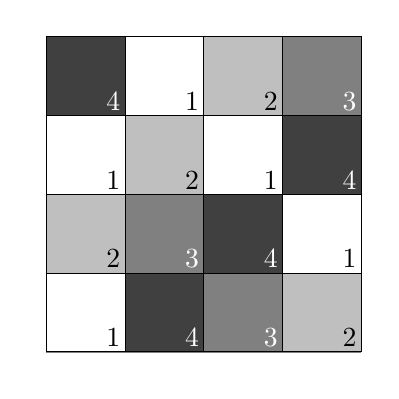
\begin{tikzpicture}
			\foreach \i in {\xMin,...,\xMax} {
				\draw [very thin,gray] (\i,\yMin) -- (\i,\yMax)
				node [below] at (\i,\yMin) {};
			}
			\foreach \i in {\yMin,...,\yMax} {
				\draw [very thin,gray] (\xMin,\i) -- (\xMax,\i)
				node [left] at (\xMin,\i) {};
			}
			\draw[fill=white]  (0, 1) -- (1, 1) -- (1,0) -- (0,0) -- cycle;
			\draw[fill=darkgray]  (1, 1) -- (2, 1) -- (2,0) -- (1,0) -- cycle;
			\draw[fill=gray]  (2, 1) -- (3, 1) -- (3,0) -- (2,0) -- cycle;
			\draw[fill=lightgray]  (3, 1) -- (4, 1) -- (4,0) -- (3,0) -- cycle;
			
			\draw[fill=lightgray]  (0, 2) -- (1, 2) -- (1,1) -- (0,1) -- cycle;
			\draw[fill=gray]  (1, 2) -- (2, 2) -- (2,1) -- (1,1) -- cycle;
			\draw[fill=darkgray]  (2, 2) -- (3, 2) -- (3,1) -- (2,1) -- cycle;
			\draw[fill=white]  (3, 2) -- (4, 2) -- (4,1) -- (3,1) -- cycle;
			
			\draw[fill=white]  (0, 3) -- (1, 3) -- (1,2) -- (0,2) -- cycle;
			\draw[fill=lightgray]  (1, 3) -- (2, 3) -- (2,2) -- (1,2) -- cycle;
			\draw[fill=white]  (2, 3) -- (3, 3) -- (3,2) -- (2,2) -- cycle;
			\draw[fill=darkgray]  (3, 3) -- (4, 3) -- (4,2) -- (3,2) -- cycle;
			
			\draw[fill=darkgray]  (0, 4) -- (1, 4) -- (1,3) -- (0,3) -- cycle;
			\draw[fill=white]  (1, 4) -- (2, 4) -- (2,3) -- (1,3) -- cycle;
			\draw[fill=lightgray]  (2, 4) -- (3, 4) -- (3,3) -- (2,3) -- cycle;
			\draw[fill=gray]  (3, 4) -- (4, 4) -- (4,3) -- (3,3) -- cycle;
			
			\node[text=black] (A1) at (0.85,0.18) {$1$};
			\node[text=white] (A1) at (1.85,0.18) {$4$};
			\node[text=white] (A1) at (2.85,0.18) {$3$};
			\node[text=black] (A1) at (3.85,0.18) {$2$};
			
			\node[text=black] (A1) at (0.85,1.18) {$2$};
			\node[text=white] (A1) at (1.85,1.18) {$3$};
			\node[text=white] (A1) at (2.85,1.18) {$4$};
			\node[text=black] (A1) at (3.85,1.18) {$1$};
			
			\node[text=black] (A1) at (0.85,2.18) {$1$};
			\node[text=black] (A1) at (1.85,2.18) {$2$};
			\node[text=black] (A1) at (2.85,2.18) {$1$};
			\node[text=white] (A1) at (3.85,2.18) {$4$};
			
			\node[text=white] (A1) at (0.85,3.18) {$4$};
			\node[text=black] (A1) at (1.85,3.18) {$1$};
			\node[text=black] (A1) at (2.85,3.18) {$2$};
			\node[text=white] (A1) at (3.85,3.18) {$3$};
		\end{tikzpicture}
		\label{subfig:RES}
	}
	
	\caption{Different clocking Schemes in QCA} \label{fig:ClockingSchemes}
\end{figure}

The tile-based clocking leads to several proposals for clocking schemes, which provide a specific distribution of clock zones. Since they follow a uniform pattern, they can be easily extended for any size of the circuit. In Figure~\ref{fig:ClockingSchemes}, three clocking schemes are shown, each based on a different idea. Since information flow is only allowed in ascending clock order modulo $clk$, the 2DDWave clocking scheme in Figure~\ref{subfig:2DD} only allows information to propagate in two directions, south and east \cite{2DD}. This simplicity prohibits back propagation, limiting the placement and routing of sequential circuits. It also restricts gates in the scheme to have a maximum input size of two, thereby not allowing the placement and routing of majority gates. The USE scheme, shown in Figure~\ref{subfig:USE}, addresses the first problem by introducing clocking loops into the scheme, providing the possibility to place sequential circuits \cite{USE}. The RES scheme, shown in Figure~\ref{subfig:RES}, addresses the second problem by giving the opportunity to place gates of input size three. Since one tile can connect to only four adjacent tiles, one of which must output the information of the gate on the tile, this gives the maximum input size allowed. This is especially important for the placement of majority gates \cite{RES}. In QCA technology, they can be represented by only one tile, making them one of the key advantages of QCA technology.

The basic building blocks of QCA have been identified and their method of data propagation through clocking has been established. With this understanding, the design and construction of QCA circuits can be undertaken. The critical aspect of this process is the proper placement and routing of these building blocks. In the following section, the placement and routing problem in QCA circuit design will be defined.

\section{Placement and routing problem} \label{sec:PR}

In this section, the placement and routing (P\&R) problem is formally defined using the theoretical foundations of gates and clocking established in the preceding sections. In simple terms, the (P\&R) problem can be formulated as the placement of logic gates, represented by vertices in a logic network, and the routing between gates via wires, represented as edges in a logic network, in a way that the logic of the logic network is retained in the designed circuit. Because each gate and its position in the layout is strongly dependent on the clocking inside the QCA domain, the circuit also has to follow two timing constraints to function correctly. In this section, the notation and constraints of placement and routing in the QCA domain are introduced. The P\&R problem, originally derived from \cite{Walter}, evolves from a grid-based tile-design in conjunction with a logic network.

\begin{definition}
	A \textit{layout} is defined by a $w \times h$ grid $\Gamma_{w, h}$ and a graph $G(V, E)$, which is placed on the grid. Each \textit{tile} of the layout can be accessed via its $x$ and $y$ coordinates. The set of tiles is denoted as $T$ with $t = (x, y) \in T$. For any vertex of the graph, $v(x, y)$ is restricted to the boundaries $x < w$ and $y < h$. For edges $\{(x, y), (x^*, y^*)\}$ it holds $\vert x-x^*\vert+\vert y-y^*\vert = 1, 0 \leq x, x^* \leq w, 0 \leq y, y^* \leq h$.
\end{definition}

\begin{definition}
	A \textit{gate-level} layout describes a layout grid in combination with a logic network $N = (\Lambda, I, \Sigma, O)$. In addition to the already known mapping \textit{placement} $p$, which assigns nodes to tiles, there are two additional mappings. The \textit{routing} $r$, which assigns logic network signals to layout paths (connected tiles) and a \textit{clocking} $c$ assigning clock numbers to tiles. The gate-level layout is therefore described as $L = (\Gamma, N, p, r, c)$.
	
	Further, nodes placed on the gate-layout are referred to as \textit{gates}. Two tiles $t_i = (x_i, y_i)$ and $t_j = (x_j, y_j)$ where $\vert x_i-x_j\vert+\vert y_i-y_j\vert = 1$ are called \textit{adjacent}. A path which is wired through adjacent tiles is called \textit{wire}. In this context, one tile corresponds to a \textit{wire segment}. If neither a gate nor a wire segment is placed on a tile, it is empty. It follows that a layout with only empty tiles is also empty. A layout is said to be S-clocked if it follows a clocking scheme S. Otherwise, it is irregularly clocked. Moreover, an adjacent tile of a tile $t \in T$, where $T$ is the set of all tiles, is incoming $t^-$ if $c(t) - c(t^-) \mod{clk} = 1$. This means that the incoming tile can forward information to the viewed tile according to pipelined clocking. For outgoing tiles $t^+$ it holds that $c(t^+) - c(t) \mod{clk} = 1$ accordingly. For QCA it was already stated that the clock number $clk = 4$.
\end{definition}

From this definition, there arise some difficulties of placing and routing a logic network onto a two-dimensional grid, with exception of wire crossings, which however are really costly and therefore should be minimized. One major challenge for P\&R algorithms is the signal synchronization, which results in a strong dependency of clocking and signal distribution. As already pointed out, for every signal path it has to hold that information can only propagate from a tile with clocking number $i$ to an outgoing tile with clocking number $(i+1 \mod clk)$. This property is called the \textit{local synchronization constraint}. The existence of possible signal paths can be assured by using predefined clocking schemes, but, however, can comprise some constraints. In addition, the \textit{global synchronization constraint} states that every two signal paths leading to the same tile must to pass the same amount of tiles starting at their primary input. Since this constraint has to hold for every gate, the complexity increases rapidly with growing network sizes. Therefore, the combination of all these challenges forms a P\&R problem, which is proven to be as $\mathcal{NP}$-complete \cite{NP-hard}.

When a gate-level layout is designed, a technology still has to be mapped onto it. To do this, the standard library proposed in Section~\ref{subsec:gates} is used for the mapping. Because the definition of the P\&R problem is based on the book \cite{Walter}, which defines it for the domain of field-coupled nanotechnologies, several FCN technologies can be mapped onto such a gate-level layout. This means that, for example, a change of clock to $clk = 3$ would also allow for placement and routing for \textit{Nanomagnet Logic} (NML)~\cite{turvani2014physical}. Therefore, although the designs in this work are only for QCA, the ideas may also apply to other FCN technologies.

\section{Sequentiality}\label{subsec:latchesandregisters}

In Section~\ref{sec:PR} about the placement and routing problem, the main constraints for the design of QCA circuits are summarized. With this knowledge, both combinational and sequential circuits can be designed and verified. Combinational circuits can be understood as a combination of logic operations, while sequential circuits additionally include the reuse of information computed by their logic, requiring a back-loop functionality. This additional back-looping is achieved through the use of storage elements, which are built according to the clocking properties of the circuit and technology. Since clocking in QCA is completely different from CMOS, storage elements and sequentiality have to be rethought. Hence, the properties of storage elements are discussed first in the CMOS domain and then transferred to the QCA domain. It should also be noted that clocking in QCA only supports synchronous information flow, which means that in the first part, only synchronous CMOS logic is considered.

\subsection{CMOS storage elements}
In order to achieve sequential behavior in CMOS technology, \textit{registers} are implemented into the circuits. A register is capable of storing and stabilizing several bits of information, which is then looped back to the logic via wires. In order to understand registers, first \textit{flip-flops}, storing each one bit and their building blocks \textit{latches} have to be discussed.

\begin{figure}
	\centering
	\begin{circuitikz}[american] \draw
		(1,0) node[not port] (not1) {}
		(1,-2) node[not port, rotate = 180] (not2) {}
		(-1,0) -- (0, 0)
		(0,0) -- (not1.in)
		(not1.out) -- (2, 0)
		(2, 0) -- (3, 0)
		(2, 0) -- (2, -2)
		(2, -2) -- (not2.in)
		(not2.out) -- (0, -2)
		(0, -2) -- (0, 0)
		
		(0.5,0) node [anchor=west] {$1$}
		(1.5,-2) node [anchor=east] {$2$}
		(-2, 0) node [anchor=west] {$in$}
		(4, 0) node [anchor=east] {$out$}
		(-2, -1) node [anchor=west] {$V_{o1}=V_{i2}$}
		(4, -1) node [anchor=east] {$V_{o2}=V_{i1}$}
		;
	\end{circuitikz}
	\caption{Eccles-Jordan-Flip-Flop}\label{fig:EJFF}
\end{figure}

The simplest storage element in CMOS, which can store one bit, is the so-called Eccles-Jordan (EJ) \text{flip-flop} (FF). It is formed by connecting the output of one inverter to the input of another inverter and vice versa. Therefore, the logic level is propagated from one inverter stage to the other, while the same value is held in it. Due to its simplicity, a high voltage shift is needed in order to change its stored value, making the FF really inert.

Also the direct connection of the input and output makes their voltage levels highly dependent on each other, which can be interpreted as noisy behavior, also referred to as \text{transparency} \cite{hawkins2012cmos}. To avoid errors caused by the transparent behavior in the transition region, the input voltage needs to be really stable. In order to receive more robust storage elements, more sophisticated ideas were implemented while preserving the general idea introduced by the EJ-FF.

By replacing the inverters in an EJ-FF with NOR gates as shown in Figure~\ref{fig:SR-Latch}, the transparency gets reduced and two inputs, a set $S$ and a reset $R$, are introduced leading to four possible input combinations and clear states. When both $S=0$ and $R=0$, the current value is latched and the storage element is in the hold state. By holding $R=0$ and changing $S=1$, the latch output is forced to $Q=1$, called the set state. Reversing both inputs to $R=1$ and $S=0$ leads to the reset state where the latch output is $Q=0$. Furthermore, with $S, R = 1$, the latch value is unstable, and therefore we get an undefined state, prohibiting this input combination. Based on its behavior, this element is called \textit{Set-Reset-Latch} (SR-Latch).

\begin{figure}
	\centering
	\begin{minipage}{0.35\textwidth}
		\begin{circuitikz}[american] \draw
			(0,2) node[nor port] (NOR1) {}
			(1,2) node[anchor=east] {Q}
			(1,0) node[anchor=east] {$\overline{Q}$}
			(0,0) node[nor port] (NOR2) {}
			(NOR1.in 1) node[anchor=east] {R}
			(NOR2.in 2) node[anchor=east] {S}
			(NOR1.out) -- ++(0,-0.5) -- ($(NOR2.in 1) +(0,0.5)$) -- (NOR2.in 1)
			(NOR2.out) -- ++(0,+0.5) -- ($(NOR1.in 2) +(0,-0.5)$)--(NOR1.in 2)
			;
		\end{circuitikz}
	\end{minipage}
	\begin{minipage}{0.35\textwidth}
		\begin{tabular}{| c | c | c | c |}
			\hline
			\textbf{S} & \textbf{R} & \textbf{$Q_{next}$} & \textbf{State}\\
			\hline
			0 & 0 & Q & hold state\\
			\hline
			0 & 1 & 0 & reset\\
			\hline
			1 & 0 & 1 & set\\
			\hline
			1 & 1 & X & undefined state\\
			\hline
		\end{tabular}
	\end{minipage}	
	\caption{SR-Latch}\label{fig:SR-Latch}
\end{figure}

In order to achieve synchronous behavior the Set and Reset inputs are clocked resulting in a gated SR-Latch. To eliminate the undefined state, the set and inverted reset inputs are connected together, forming the D-Latch shown in Figure~\ref{fig:D-Latch}. Consequently, a value is held if the clock $clk=0$ and the D lock propagates the input value $D$ if $clk=1$. To give a memory element the ability to clock Boolean operations from one stage to another, \emph{edge-triggered} flip flops are introduced. Rising clock edges determine when the FF overwrites and passes its data. An edge-triggered \emph{Data FF} (D-FF) can be constructed by connecting two D-latch stages behind each other. The first stage is activated at rising edges, while the second stage is activated at falling clock edges. In this way, the D-FF takes new data at a rising edge and passes them in the next clock cycle from its output. Also, the edge-triggered FF eliminates the transparency. Regarding the term edge-sensitive for D-FFs, latches are considered to be level-sensitive \cite{hawkins2012cmos}.\\

\begin{figure}
	\centering
	\begin{minipage}{0.5\textwidth}
		\begin{circuitikz}[american] \draw
			% Draw and gates
			(0,2) node[and port] (and1) {}
			(0,0) node[and port] (and2) {}
			
			% Draw nor gates
			(and1.out) -- ++(0.25,0) node
			[
			nor port,
			anchor=in 1
			] (nor1) {}
			
			(and2.out) -- ++(0.25,0) node
			[
			nor port,
			anchor=in 2
			] (nor2) {}
			
			(nor1.in 2) -| ++ (-0.3,-0.25) -- ++(2,-0.5) coordinate(a) |- (nor2.out)
			(nor2.in 1) -| ++ (-0.3,0.25) -- ++(2,0.5) |- (nor1.out)
			
			% Clock
			(and1.in 2) -- (and2.in 1)node[midway](clk){}
			(clk.center) -- ++(-1.25,0) node[left]{Clk}
			
			% Output labels
			(nor1.out -| a) -- ++(0.75,0) node[right]{$Q$}
			(nor2.out -| a) -- ++(0.75,0) node[right]{$\overline{Q}$}
			
			(and2.in 2) -- ++(-1.25,0) coordinate(a2) node[left=0.1cm]{D}
			
			% Not port
			(-1.9,0.2) node
			[
			not port,
			rotate=90,
			scale=0.5,
			](not) {}
			
			(not.in) |- (a2) (not.out) |- (and1.in 1)  
			;
		\end{circuitikz}
	\end{minipage}
	\begin{minipage}{0.4\textwidth}
		\begin{tabular}{| c | c | c | c |}
			\hline
			\textbf{clk} & \textbf{D} & $Q_{next}$ & \textbf{State}\\
			\hline
			0 & 0 & * & hold state\\
			\hline
			0 & 1 & 0 & propagate\\
			\hline
			1 & 0 & 1 & propagate\\
			
			\hline
		\end{tabular}
	\end{minipage}	
	\caption{D-Latch}\label{fig:D-Latch}
\end{figure}

\subsection{QCA storage elements}

The goal of a storage element in QCA is to have all the properties of a D-FF, so it can store data from one clock cycle and pass it to the combinational logic in the next clock cycle. Also the element should not be transparent and the effect of an edge triggered element has to be discussed. In the QCA ONE library an effort was made to translate the D-FF into QCA by just replacing the CMOS gates and wires with the corresponding QCA gates. Thus a second external $clk$ signal is introduced, mimicking the clock of a CMOS circuit. But since the QCA circuit already has its own clock with a dependency on all gates of the circuit and the clocking has some major differences CMOS, as already observed in Section~\ref{subsec:clocking}, this implementation is questionable and the implementation of latches and FFs in QCA has to be rethought from scratch.

This leads us to ideas to look at QCA storage elements dependent on their corresponding clocking.
The effort of rethinking storage elements in QCA from scratch was already made in \cite{torres2018synchronization}. The proposed solution to create a QCA element which is able to store one bit is rather simple. Since every tile is clocked on its own, a simple latch can be formed by a wire segment, held in the hold phase of the clocking, as shown in Figure~\ref{subfig:Wire_FF}. In Figure~\ref{fig:sequ_el_clocking} the clocking of this wire segment is depicted. The data is propagating into the latch and by holding the hold phase by exactly one clock cycle the data is passed to the next logic block exactly one clock cycle later. Also the question arises if this element is a level-sensitive latch or if it is a edge-sensitive FF. For the latch we could argue that the information is clearly not sampled at one time point like in an ideal FF, but rather the information is taken into the latch during the whole switch phase. On the other hand one could argue that the switch phase could be seen like a real-time rising clock edge, where the data is sampled and then held while the clock is in hold phase or "1". For this work, the comparison to a FF seems to be more suited because also no transparency is allowed due to the strictly independent clocked tiles in QCA. The only functionality that the wire-FF misses is a set-reset option. The concept of replacing wire with a majority gate while maintaining the same clocking was also proposed in \cite{Walter}. Now the D-FF basically has the same functionality but has two external inputs which can force the gate to zero by setting both inputs to zero or force the gate to one by setting both inputs to one. In the other configurations, the majority-FF would act as normal storage element. Figure~\ref{subfig:Maj_FF} shows such a D-FF.

\begin{figure}
	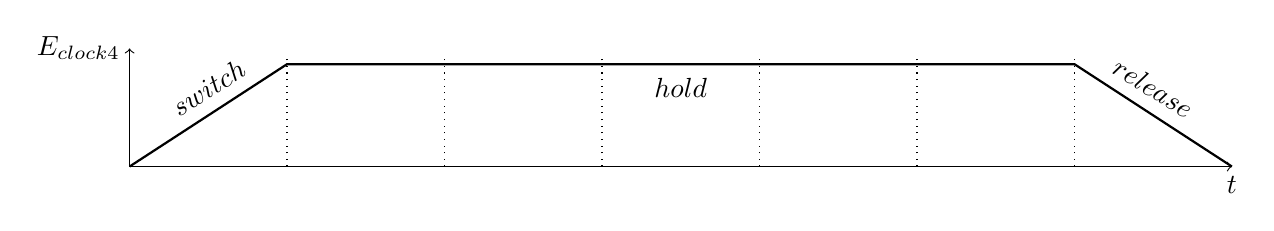
\begin{tikzpicture}
		
		% horizontal axis
		\draw[->] (0,0) -- (14,0) node[anchor=north] {$t$};
		
		% vertical axis
		\draw[->] (0,0) -- (0,1.5) node[anchor=east] {$E_{clock4}$};
		% nominal speed
		\draw[dotted] (2,0) -- (2,1.4);
		\draw[dotted] (4,0) -- (4,1.4);
		\draw[dotted] (6,0) -- (6,1.4);
		\draw[dotted] (8,0) -- (8,1.4);
		\draw[dotted] (10,0) -- (10,1.4);
		\draw[dotted] (12,0) -- (12,1.4);
		
		% Us
		\draw[thick] (0,0) -- (2,1.3) -- (4,1.3) -- (6,1.3) -- (8,1.3) --  (10,1.3) -- (12, 1.3) -- (14, 0);
		\draw (1,1.4) node {}; %label
		\draw (1,1) node [rotate = 32] {$switch$};
		\draw (7,1) node [] {$hold$};
		\draw (13,1) node [rotate = -32] {$release$};
		
	\end{tikzpicture}
	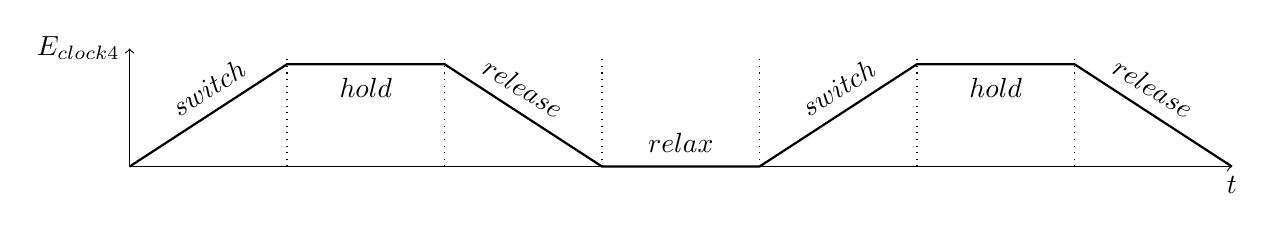
\begin{tikzpicture}
		
		% horizontal axis
		\draw[->] (0,0) -- (14,0) node[anchor=north] {$t$};
		
		% vertical axis
		\draw[->] (0,0) -- (0,1.5) node[anchor=east] {$E_{clock4}$};
		% nominal speed
		\draw[dotted] (2,0) -- (2,1.4);
		\draw[dotted] (4,0) -- (4,1.4);
		\draw[dotted] (6,0) -- (6,1.4);
		\draw[dotted] (8,0) -- (8,1.4);
		\draw[dotted] (10,0) -- (10,1.4);
		\draw[dotted] (12,0) -- (12,1.4);
		
		% E
		\draw[thick] (0,0) -- (2,1.3) -- (4,1.3) -- (6,0) -- (8,0) --  (10,1.3) -- (12,1.3) -- (14,0);
		\draw (1,1.4) node {}; %label
		\draw (1,1) node [rotate = 32] {$switch$};
		\draw (3,1) node [] {$hold$};
		\draw (5,1) node [rotate = -32] {$release$};
		\draw (7,0.3) node [] {$relax$};
		\draw (9,1) node [rotate = 32] {$switch$};
		\draw (11,1) node [] {$hold$};
		\draw (13,1) node [rotate = -32] {$release$};
	\end{tikzpicture}
	\caption{Clocking of a basic latch in QCA}\label{fig:sequ_el_clocking}
\end{figure}

\begin{figure}
	\centering
	\subfigure[Wire FF]{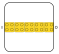
\includegraphics[scale=0.7]{wire_FF}\label{subfig:Wire_FF}}\qquad
	\subfigure[D-FF]{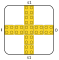
\includegraphics[scale=0.7]{maj_FF}\label{subfig:Maj_FF}}
	\caption{QCA storage elements} \label{fig:QCAFFs}
\end{figure}